\documentclass[11pt]{article}
\usepackage[margin=1in]{geometry}
\usepackage[T1]{fontenc}
\usepackage[utf8]{inputenc}
\usepackage{lmodern}
\usepackage{booktabs}
\usepackage{enumitem}
\usepackage{hyperref}
\usepackage{graphicx}
\usepackage[
  backend=biber,
  style=numeric,
  sorting=none,
  giveninits=true,
  maxbibnames=3,
  minbibnames=1,
  maxcitenames=2,
  doi=false,
  url=false,
  isbn=false,
  eprint=false
]{biblatex}
\usepackage[fontset=fandol]{ctex}

\addbibresource{zzzaurak.bib}

\hypersetup{hidelinks}

\newcommand{\code}[1]{\texttt{#1}}

\title{观测天体物理 2026 P2Rp4：超新星数据分析报告}
\author{第一组}
\date{2026年6月3日}

\begin{document}
\maketitle

\section*{分工贡献}
\addcontentsline{toc}{section}{分工贡献}
\medskip
\noindent\begin{tabular}{p{0.28\linewidth}p{0.20\linewidth}p{0.44\linewidth}}
\toprule
任务 & 负责人 & 贡献内容 \\
\midrule
引言、科学背景 & Linlin & \dots \\

目标选取与观测准备 & Minxuan He & \dots \\

数据约化与分析 & Ziheng Zhang & 整理学长提供的一维 BFOSC 光谱，完成 TNS 红移整理、稀疏光谱谱线测量、质量控制表格、诊断图和 TARDIS 定性比较。 \\

结果与结论（及总结） & Xinyu Liu & \dots \\

\bottomrule
\end{tabular}

\tableofcontents
\newpage

\section{科学问题}

\section{数据}

\section{数据处理与分析方法}
分析从项目中的一维 BFOSC 光谱 FITS 文件开始，共包含 5 个目标、12 条光谱。除每颗超新星最后一条光谱来自我们 2026 年 5 月 8 日使用兴隆 2.16 米望远镜观测外，其余历元为黄睿丰学长交付给我们的已归约数据。因此，本工作没有从二维谱重新完成 bias/flat 校正、宇宙线剔除、二维波长定标、天空扣除和一维抽取；这些基础归约步骤已在数据交付前完成。

BFOSC 是兴隆 2.16 米望远镜的常用低分辨率成像与光谱仪，典型低分辨率光谱分辨率约为 $R\sim500$--$2000$ \cite{fanXinglong216m2016,zhaoBFOSCEfficiency2018}。王晓锋老师团队的清华超新星光谱数据发布工作提供了一个与本项目最接近的参照：其 Type II 超新星光谱样本包含大量兴隆 2.16 米望远镜和丽江 2.4 米望远镜获得的光谱，并对谱线识别、速度和 pEW 等量进行系统测量 \cite{linSpectralDataRelease2024}。参照这类工作，常规长缝超新星光谱归约通常包括 CCD 本底和坏点处理、平场校正、弧灯波长定标、天空背景扣除、一维抽取、标准星或仪器响应给出的相对流量校正，以及必要时的大气吸收或相对响应修正。本项目使用的是这些步骤之后的一维光谱，因此我们后续分析的不确定性不包含完整的原始归约误差。

目标类型、发现日期和红移优先来自 TNS 的公开数据集。本项目不再手动测红移；当前 TNS 数据没有 maximum light 或 peak date 字段，因此本文中的相位均为距发现日天数，不是相对最大光相位。对有 TNS 红移的目标，将观测波长按
\[
\lambda_{\rm rest}=\frac{\lambda_{\rm obs}}{1+z_{\rm TNS}}
\]
转到静止系。SN2026LMP 在 TNS 中缺少可靠红移，因此只做定性线型检查，不采用任何定量速度或 pEW 结论。

项目程序详见 \url{https://github.com/Zzzaurak/obsastro-sn-pipeline}。本节主要分析由 \path{src/spectral_pipeline.py} 和 \path{src/spectral_notebook_tools.py} 实现，\path{notebooks/02_spectral_analysis_pipeline.ipynb} 作为交互检查界面。流程的分类和模板比较思想参考 SNID 与 WISeREP 等公开光谱比较工作 \cite{blondinDeterminingTypeRedshift2007,yaronWISeREPInteractiveSupernova2012}。

\subsection{类型、红移和最终线表选择}
为了避免弱线、混合线和缺红移目标进入定量结论，本次重新校对后采用更保守的线表。Ia 型目标 SN2026FVX 和 SN2026JLM 采用 Ca II H\&K 与 Si II 6355；Si II 5972 对局部窗口非常敏感，容易被 Si II 6355 的宽吸收污染 pEW，因此不列入最终采用表。SN2026KID 为 Type II，只采用 Fe II 5169 作为速度量级指标；H$\alpha$/H$\beta$ 在本批光谱中受 P-Cygni 发射结构、噪声和局部连续谱影响，不作为自动采用速度。SN2026KIE 为单历元 SN Ic，采用 Ca II H\&K、Ca II NIR 和 O I 7774，但 Ca II NIR 较浅，解释时只作为辅助。SN2026LMP 粗分类接近 SN IIb，但缺少 TNS 红移，因此所有候选线均保留为 \code{check}。

\begin{table}[htbp]
\centering
\caption{本节采用的目标级状态和最终线表。相位为距 TNS 发现日天数。}
\label{tab:target-status}
\resizebox{\linewidth}{!}{%
\begin{tabular}{llcccl}
\toprule
目标 & 类型 & 红移 & 光谱数 & 相位范围（天） & 采用谱线 \\
\midrule
SN2026FVX & SN Ia & 0.004846 & 4 & 1.7--51.6 & CaIIHK, SiII6355 \\
SN2026JLM & SN Ia & 0.016738 & 3 & 14.5--26.6 & CaIIHK, SiII6355 \\
SN2026KID & SN II & 0.0017 & 3 & 4.0--16.1 & FeII5169 \\
SN2026KIE & SN Ic & 0.00424 & 1 & 16.3--16.3 & CaIIHK, CaIINIR, OI7774 \\
SN2026LMP & SN IIb & -- & 1 & -- & none \\
\bottomrule
\end{tabular}}
\end{table}

\begin{figure}[htbp]
\centering
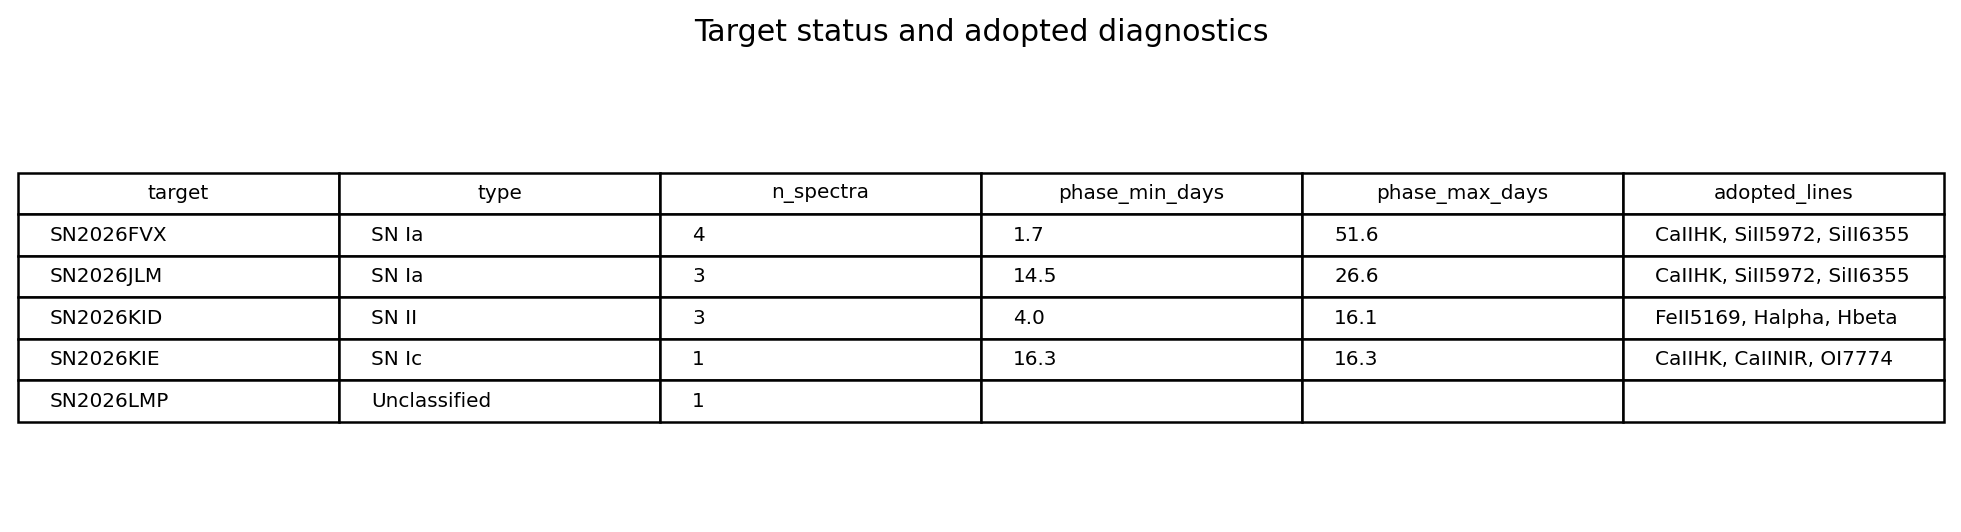
\includegraphics[width=0.96\linewidth]{images_zzzaurak/target_status_table.png}
\caption{目标级状态表。SN2026LMP 因缺少可靠 TNS 红移，只保留定性检查，不进入速度或 pEW 的定量结论。}
\label{fig:target-status}
\end{figure}

\subsection{谱线测量算法}
每条待测吸收线在静止系中截取局部窗口，先用 Savitzky--Golay 平滑压低像素噪声，再用窗口两侧的中位数点定义局部线性连续谱。归一化谱为
\[
f_{\rm norm}(\lambda)=\frac{f_{\rm smooth}(\lambda)}{f_{\rm cont}(\lambda)}.
\]
根据杨轶老师的建议，不再用高斯轮廓拟合吸收线中心，而是在归一化谱中直接取吸收最低点：
\[
\lambda_{\rm min}=\arg\min f_{\rm norm}(\lambda).
\]
速度和线深定义为
\[
v=c\frac{\lambda_0-\lambda_{\rm min}}{\lambda_0}, \qquad
d=1-f_{\rm norm}(\lambda_{\rm min}),
\]
其中 $\lambda_0$ 为实验室静止波长。FWHM 是在半深度水平
\[
f_{1/2}=1-\frac{d}{2}
\]
左右寻找线性交点 $\lambda_{\rm L}$ 和 $\lambda_{\rm R}$，定义
\[
{\rm FWHM}=\lambda_{\rm R}-\lambda_{\rm L}.
\]
pEW 直接积分归一化谱中低于连续谱的正面积：
\[
{\rm pEW}=\int_{\lambda_1}^{\lambda_2}\max\left[1-f_{\rm norm}(\lambda),0\right]\,d\lambda.
\]
这种最低点法比旧的高斯中心更直接，也更接近我们人工检查宽吸收谷时的判断方式。Ia 型目标的 Si II 和 Ca II 速度、pEW 主要用于和 BSNIP/CSP 等样本比较 \cite{silvermanBerkeleySupernovaIa2012a,folatelliSPECTROSCOPYTYPEIa2013,zhaoInvestigationFWHMAbsorption2026}；Type II 和贫包层目标则参考 Type II 与 stripped-envelope 光谱样本 \cite{gutierrezTypeIISupernova2017,linSpectralDataRelease2024,modjazOPTICALSPECTRA732014,xiangSpectralDatasetStrippedenvelope2026}。

误差棒是形式统计误差。速度误差由最低点波长不确定度传播；最低点波长不确定度由局部残差噪声和像素采样共同估计。pEW 误差由局部归一化残差噪声在吸收积分区内传播。FWHM 误差是半深度交点附近的采样级估计。此外还有 \code{velocity\_sys\_kms}、\code{pEW\_sys\_A}、\code{FWHM\_sys\_A}，记录改变平滑窗口和连续谱边缘比例后的经验散布。这些仍不是完整误差预算，没有完全包含 TNS 红移误差、波长定标系统误差、线混合和大气/仪器响应。

\subsection{人工校对和最终采用规则}
自动测量后，我们逐个查看了每个目标的局部诊断图。图中灰线为原始局部谱，黑线为平滑谱，橙线为局部连续谱，红虚线为实验室静止波长，绿虚线为本次采用的吸收最低点，紫色填充只表示 pEW 积分区域，不是高斯模型。

人工校对主要做了三类处理：第一，删除或降权容易混线的谱线，例如 Si II 5972 的 pEW 容易混入 Si II 6355，因此从最终采用表中移除。第二，删除不稳的氢线自动速度，SN2026KID 的 H$\alpha$/H$\beta$ 局部最低点受发射峰、噪声和连续谱影响，不作为 adopted 速度。第三，缺红移目标不做定量采用，SN2026LMP 即使有候选线，也因为缺少 TNS 红移全部标为 \code{check}。

最终 \path{line_diagnostics_qc.csv} 共有 28 条候选测量，其中 18 条为 \code{adopt}、10 条为 \code{check}。自动最低点明显不可靠的窄谷已经由 QC 留在 \code{check}，包括 SN2026FVX 2026-03-26 的 Ca II H\&K、SN2026JLM 2026-05-04 的 Ca II H\&K，以及 SN2026LMP 的所有缺红移候选线。

具体来说，SN2026KID 的 Fe II 5169 三个 \code{adopt} 点线深较浅，SN2026KIE 的 Ca II NIR pEW 误差大于测量值，SN2026FVX/SN2026JLM 早期 Ca II H\&K 的 pEW 也受连续谱选择影响较大。这些点仍可作为速度量级或 line ID 支持，但不适合对 pEW 或 FWHM 做强物理解释。若后续要得到更严格的最终表，可以在 QC 中加入 pEW 信噪比或 systematics 阈值，把这些弱 \code{adopt} 行降为 \code{check}；代价是 Ia 早期 Ca II 和 core-collapse 速度覆盖会更少。

\begin{figure}[htbp]
\centering
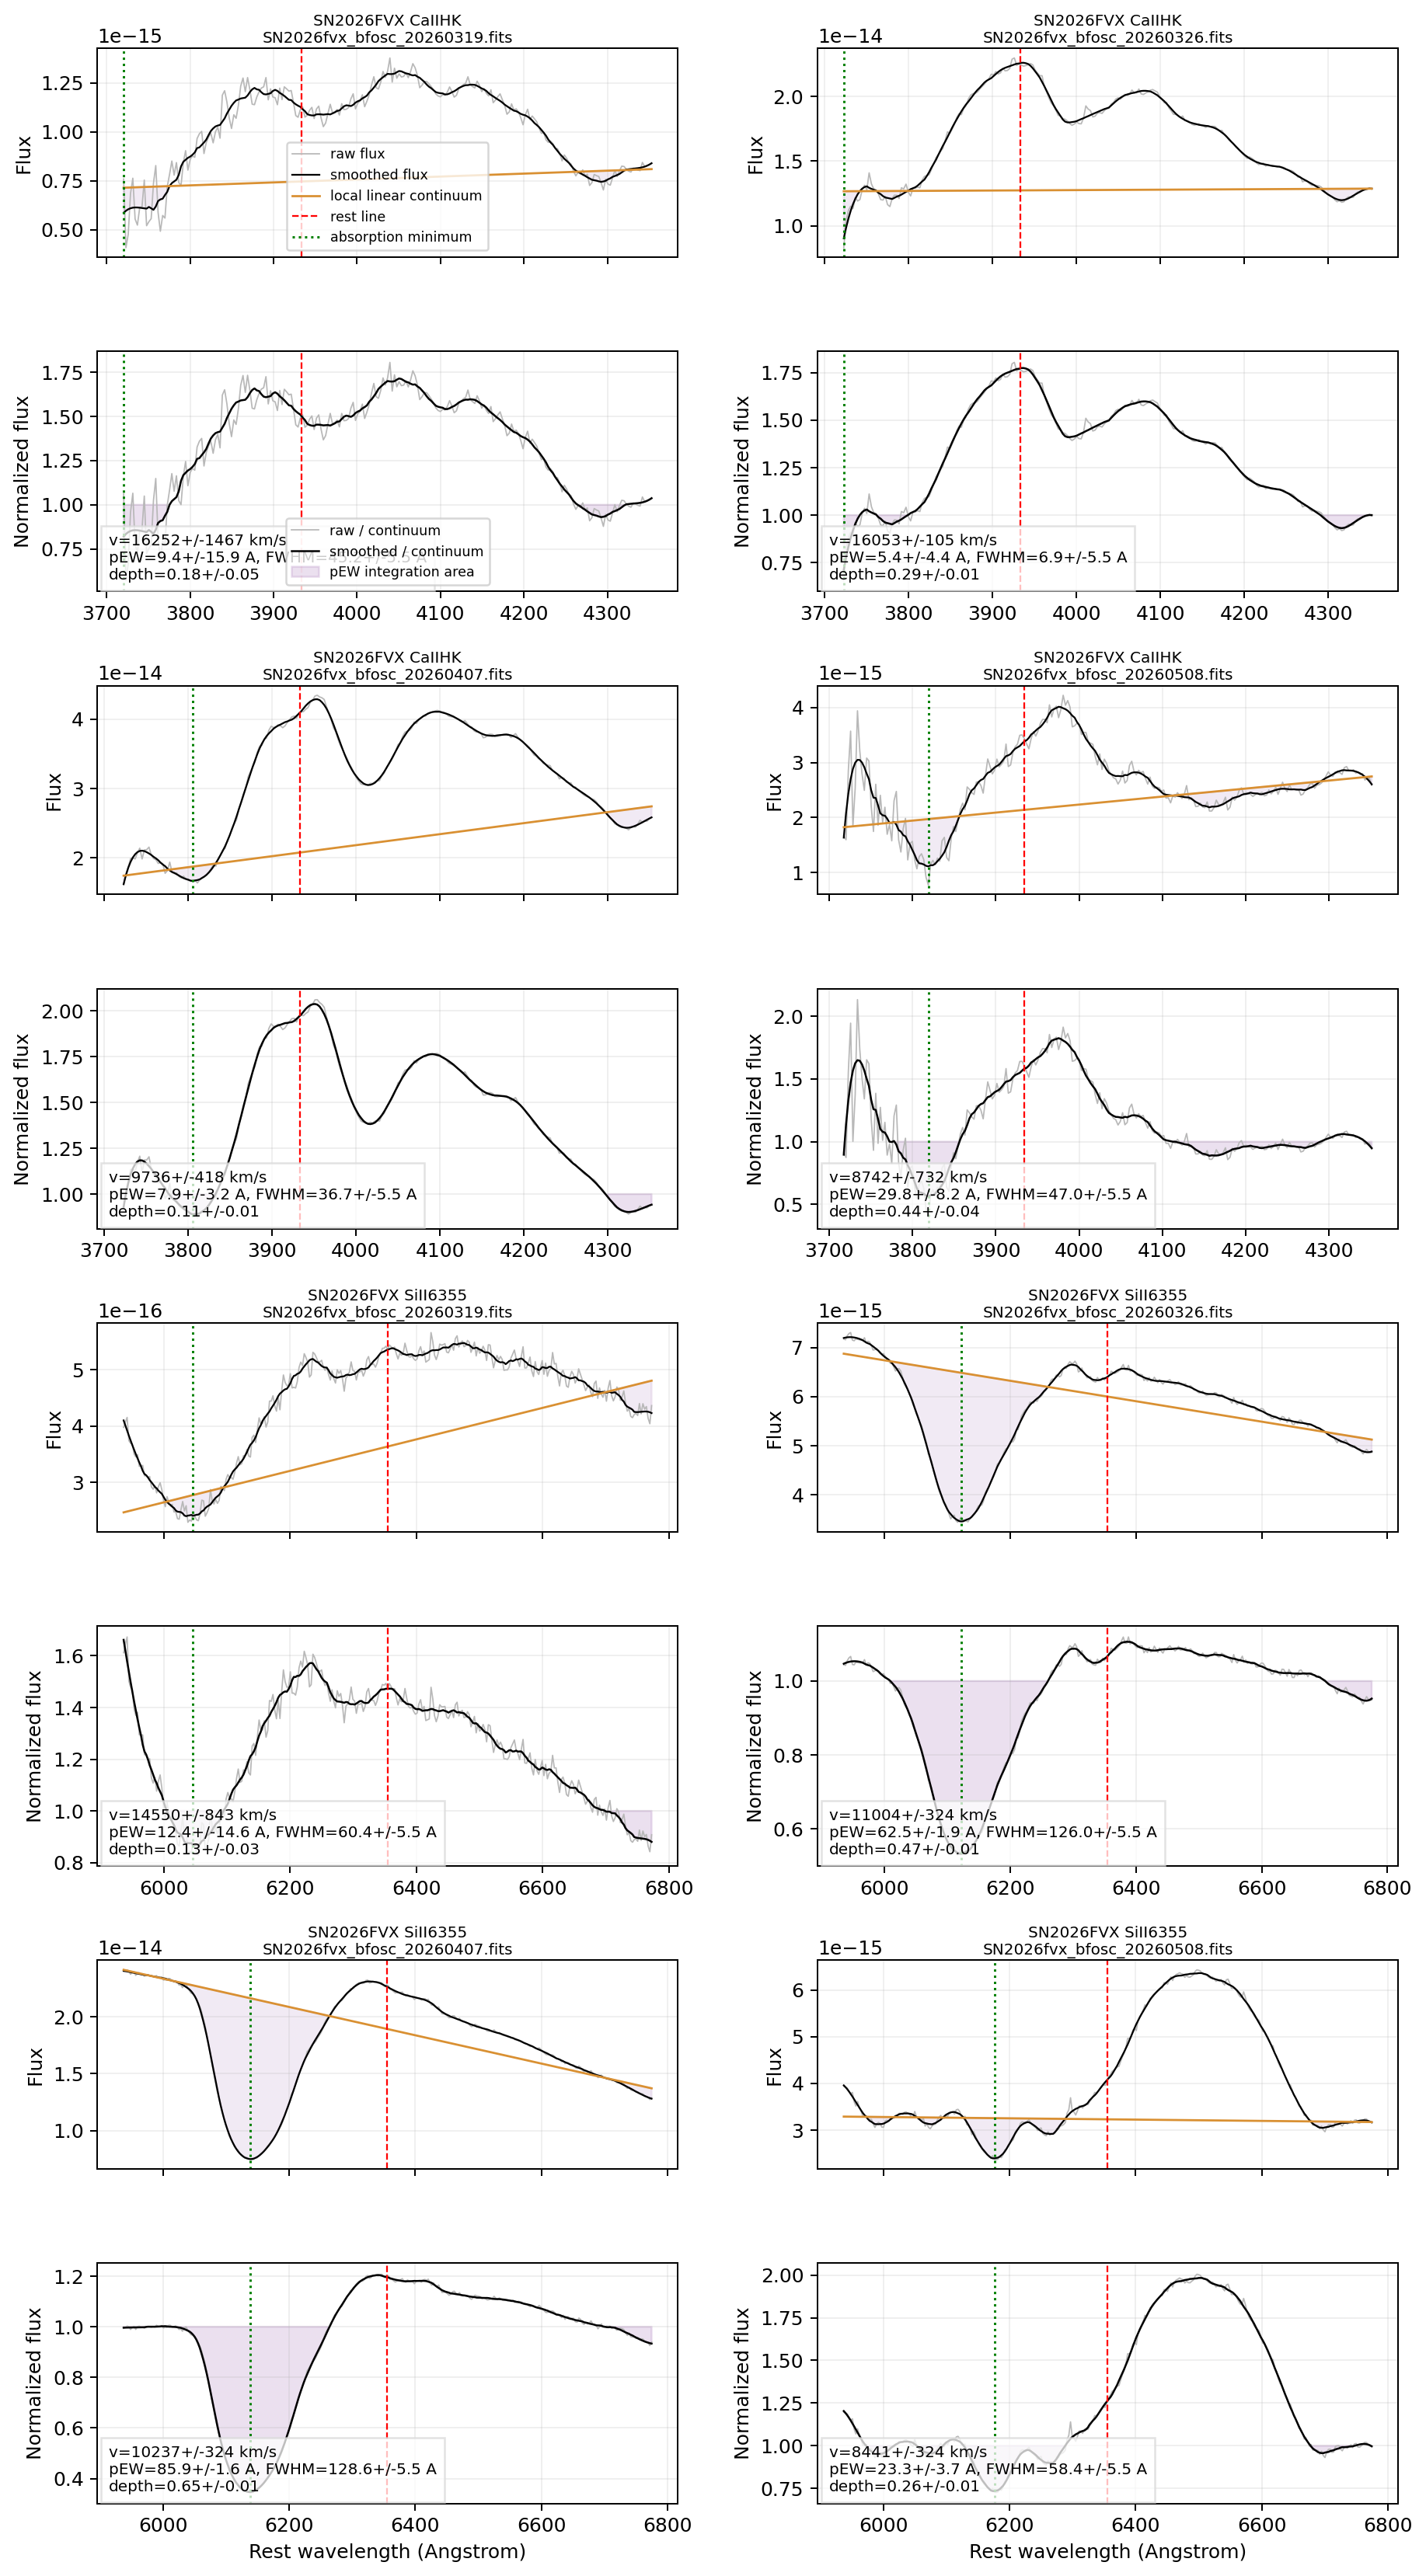
\includegraphics[width=0.96\linewidth,height=0.68\textheight,keepaspectratio]{images_zzzaurak/SN2026FVX_line_diagnostics_grid.png}
\caption{SN2026FVX 的局部谱线诊断图。绿色虚线为最低点法采用的吸收中心，紫色区域为 pEW 积分区域。}
\label{fig:fvx-line-grid}
\end{figure}

\begin{figure}[htbp]
\centering
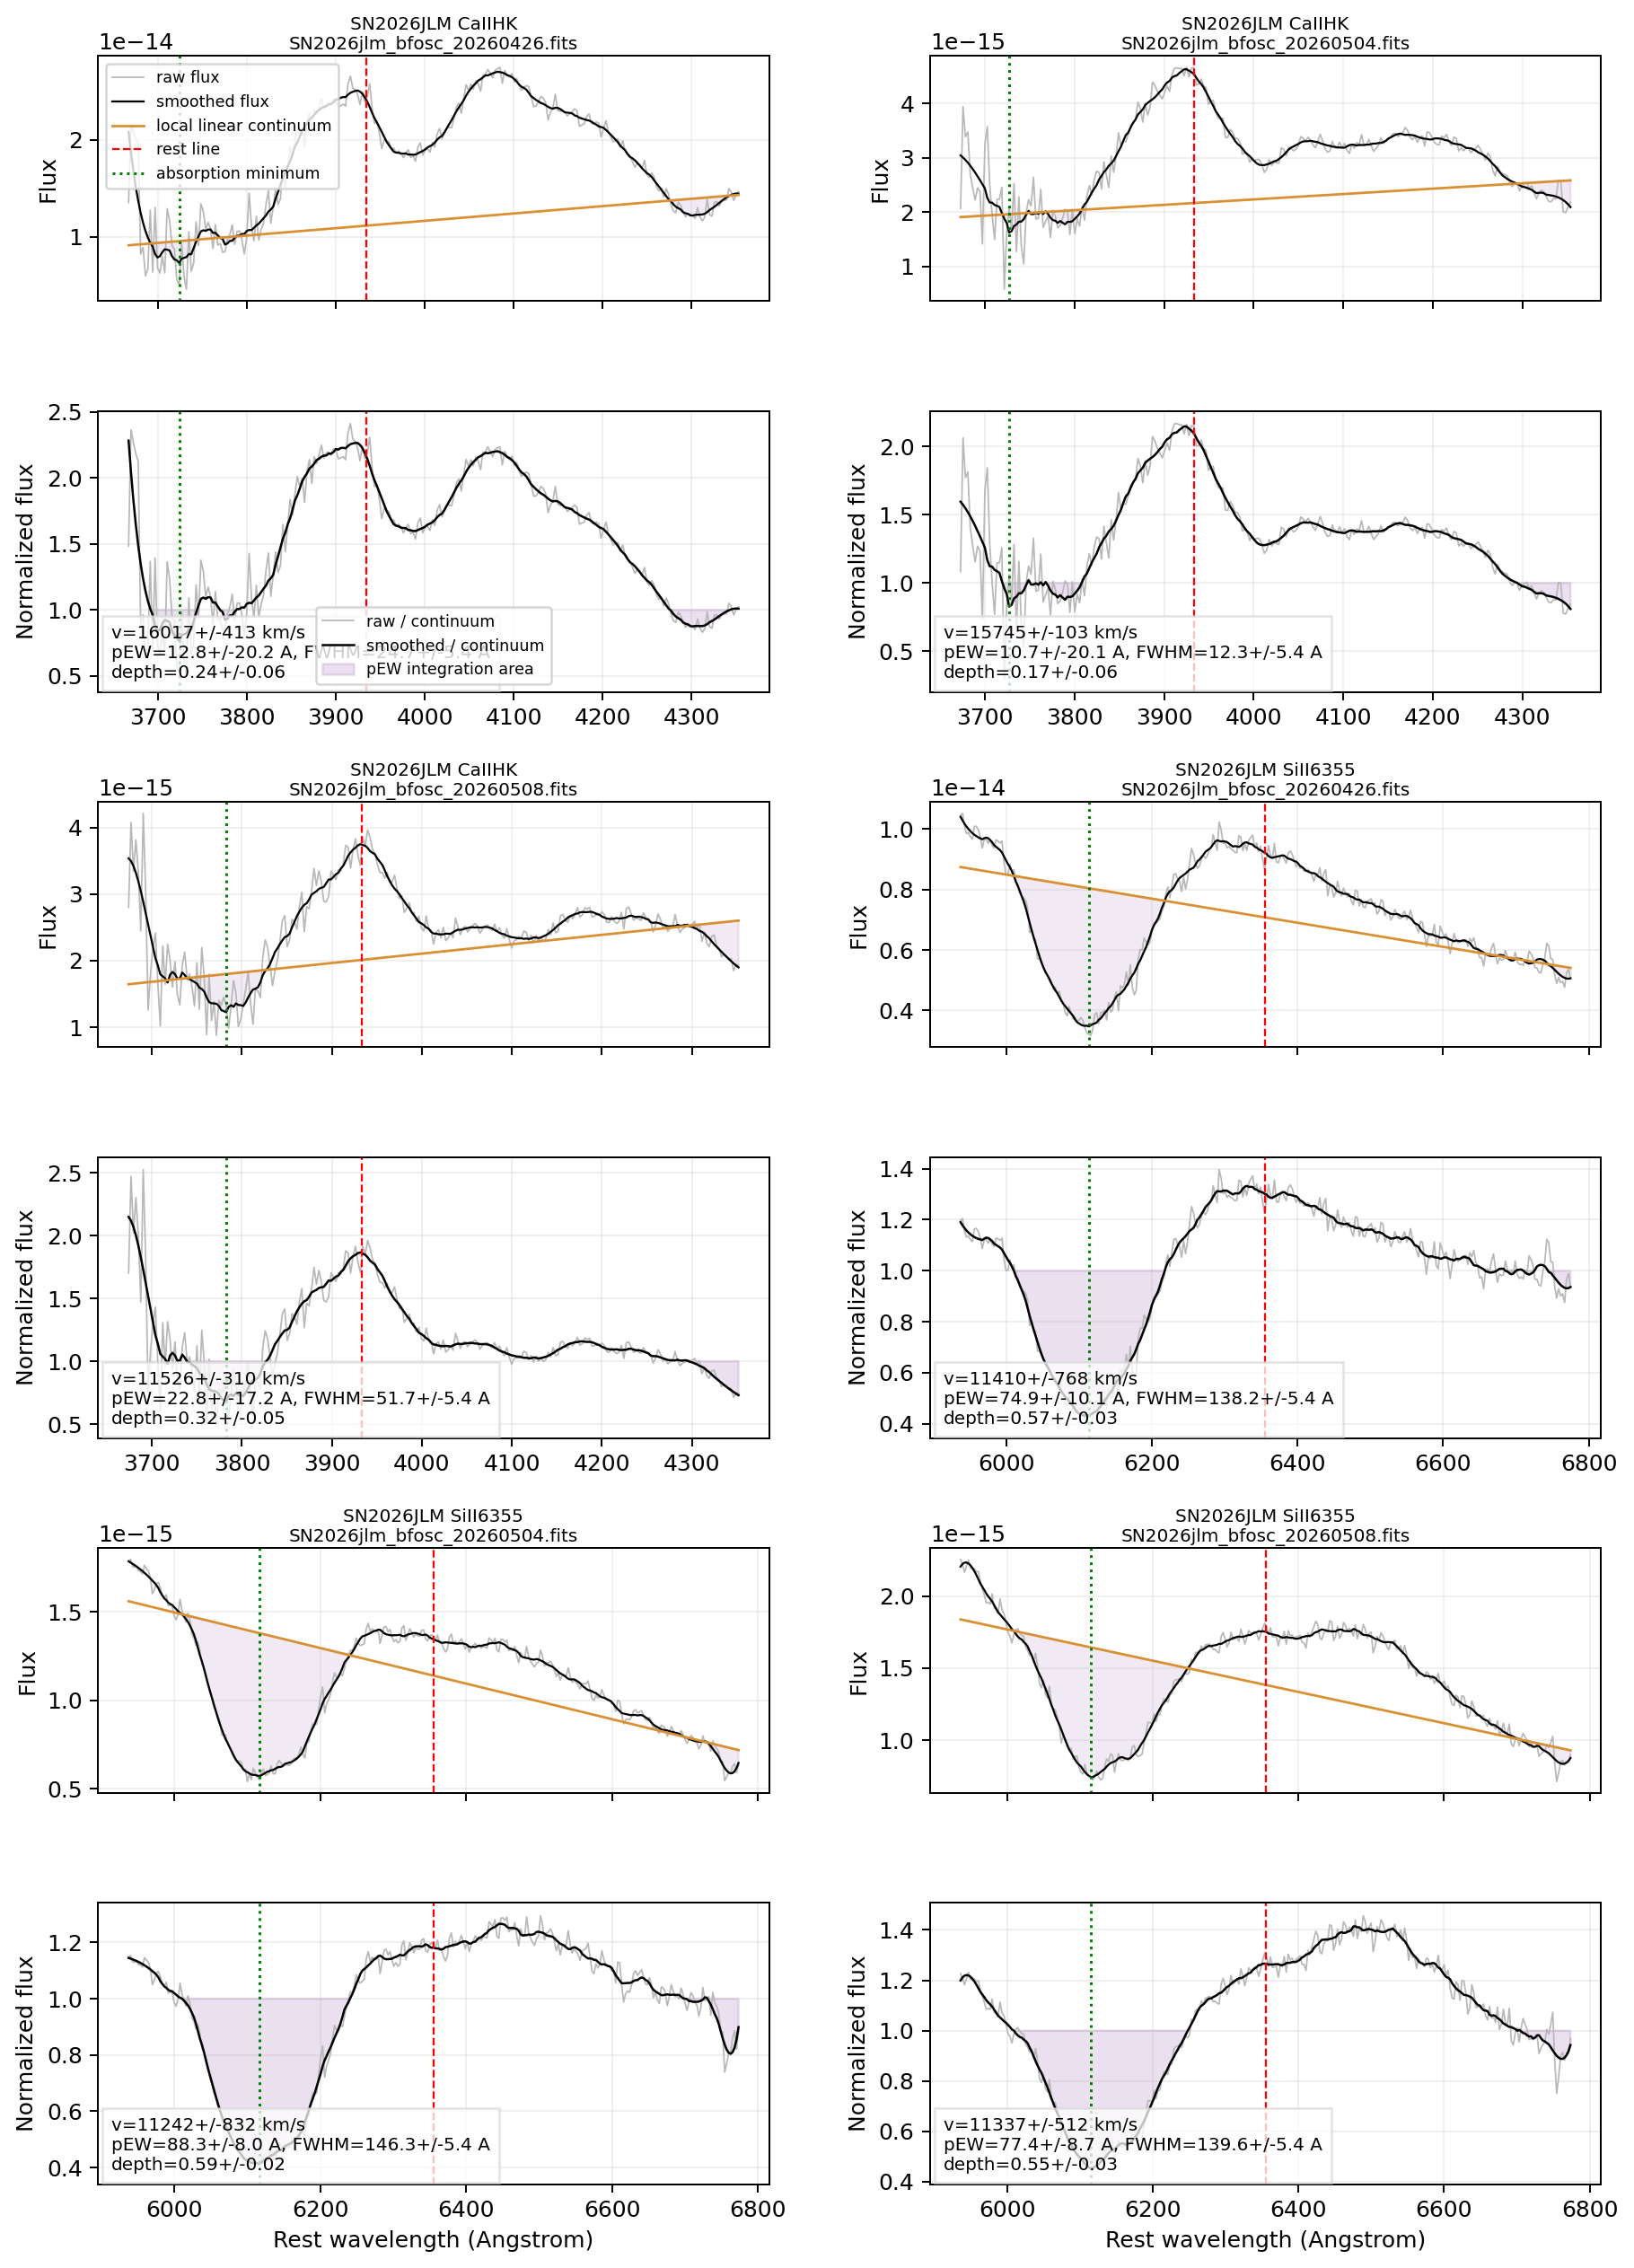
\includegraphics[width=0.96\linewidth,height=0.68\textheight,keepaspectratio]{images_zzzaurak/SN2026JLM_line_diagnostics_grid.png}
\caption{SN2026JLM 的局部谱线诊断图。Si II 6355 是本目标最稳定的 Ia 速度指标。}
\label{fig:jlm-line-grid}
\end{figure}

\begin{figure}[htbp]
\centering
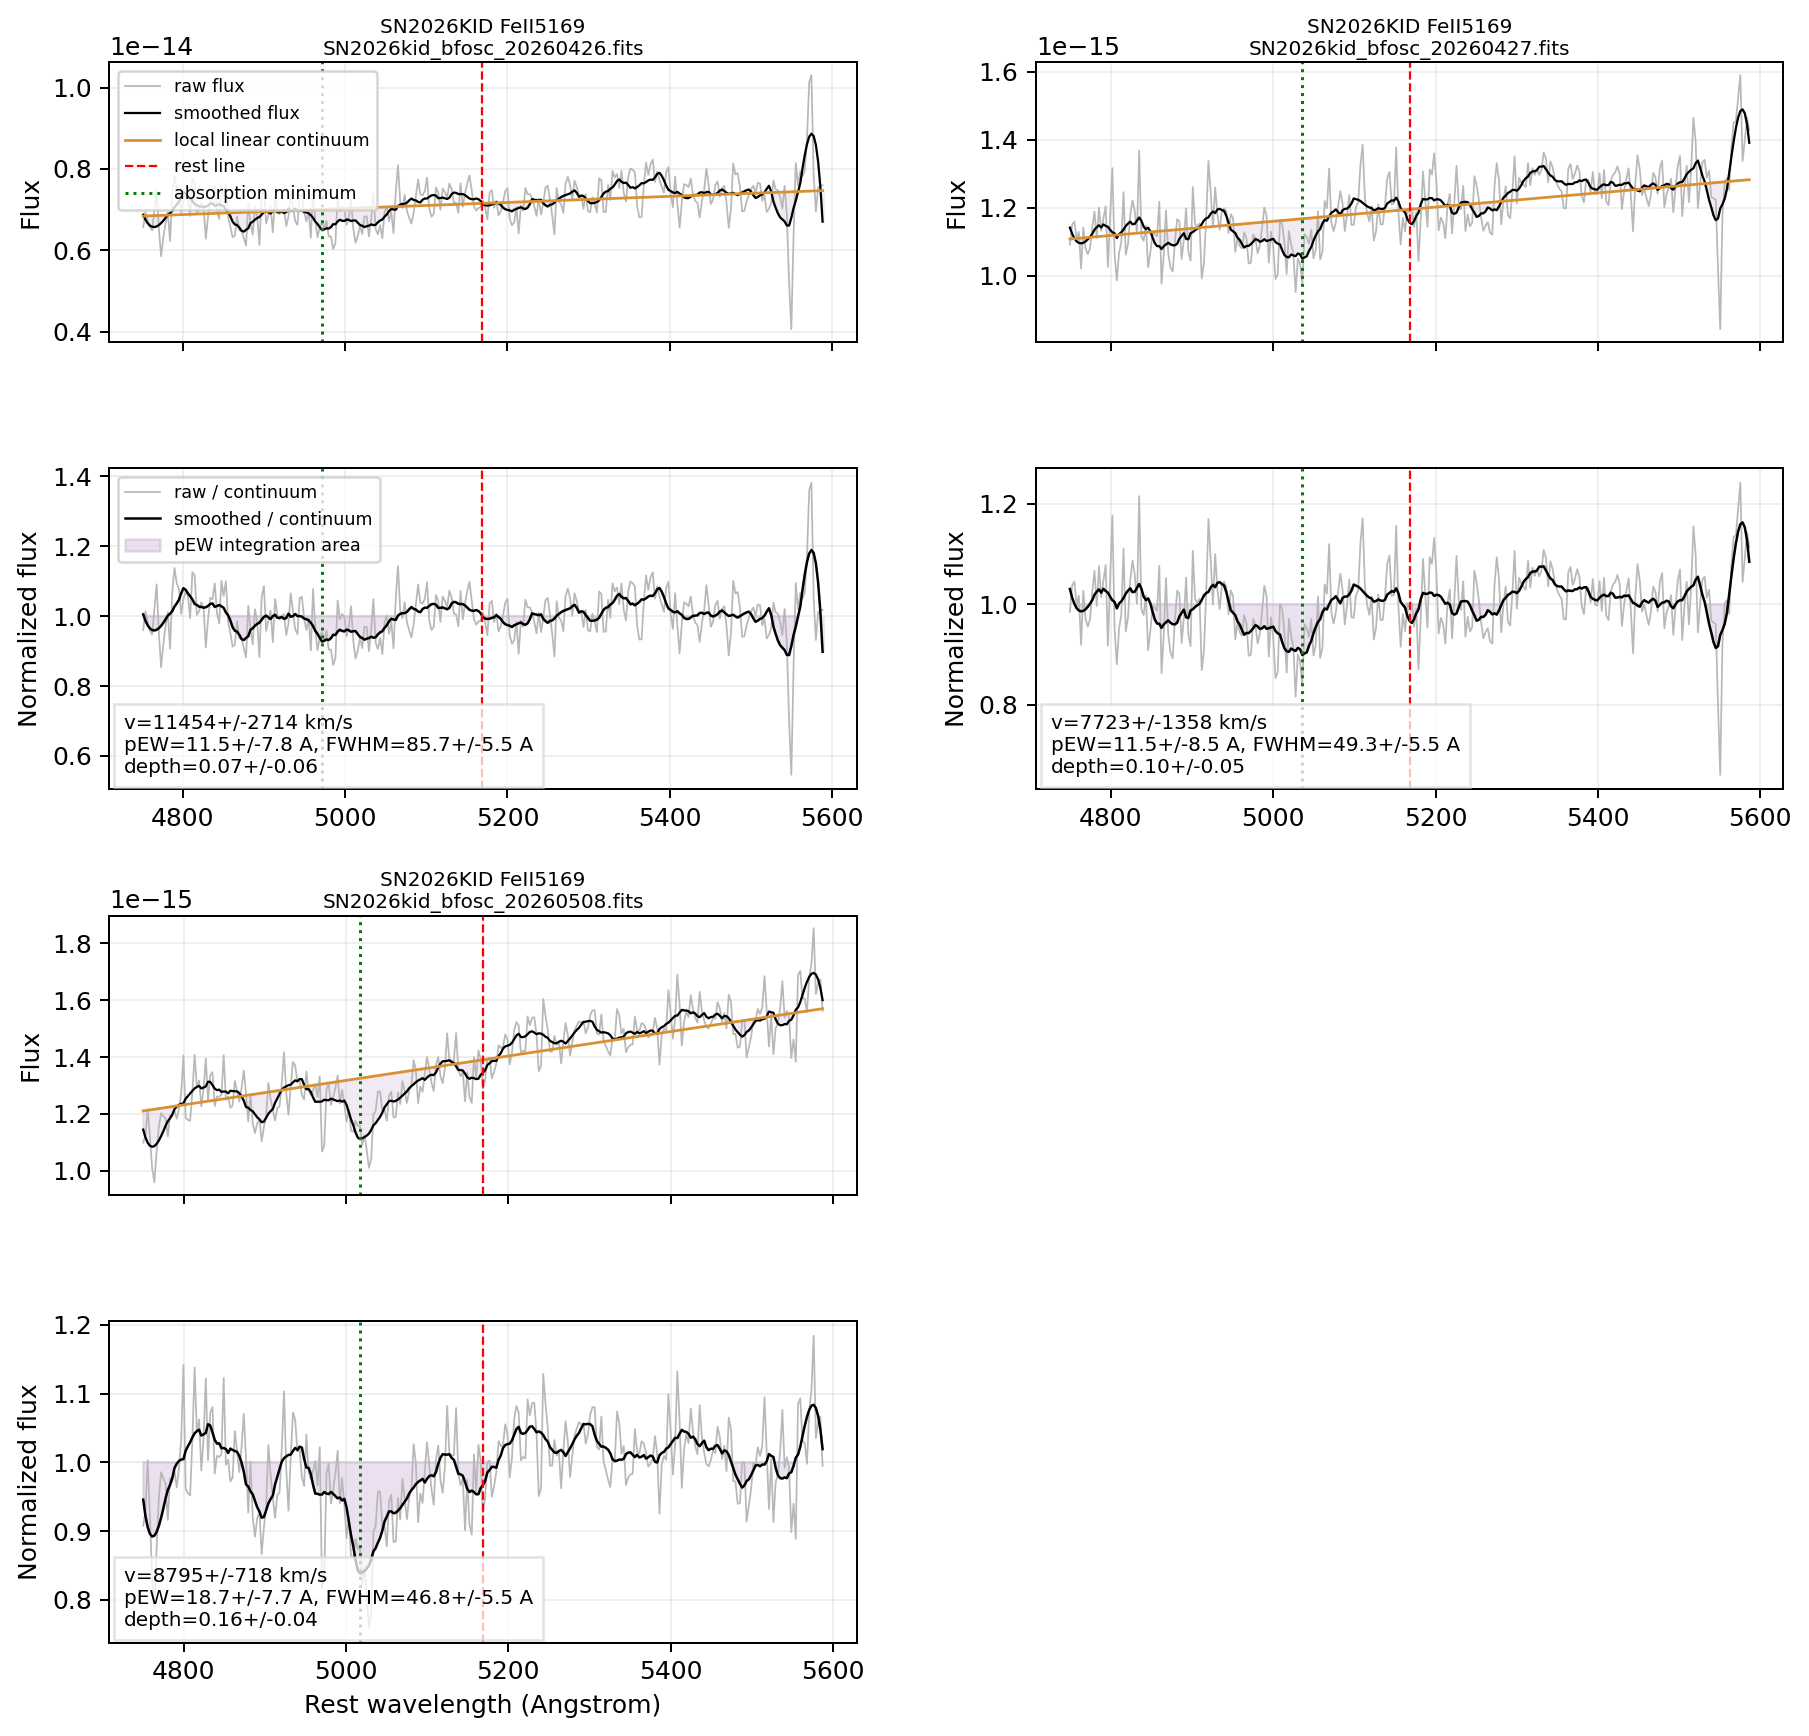
\includegraphics[width=0.96\linewidth,height=0.68\textheight,keepaspectratio]{images_zzzaurak/SN2026KID_line_diagnostics_grid.png}
\caption{SN2026KID 的局部谱线诊断图。最终只采用 Fe II 5169 作为 Type II 速度量级指标，Balmer 线仅作形态检查。}
\label{fig:kid-line-grid}
\end{figure}

\begin{figure}[htbp]
\centering
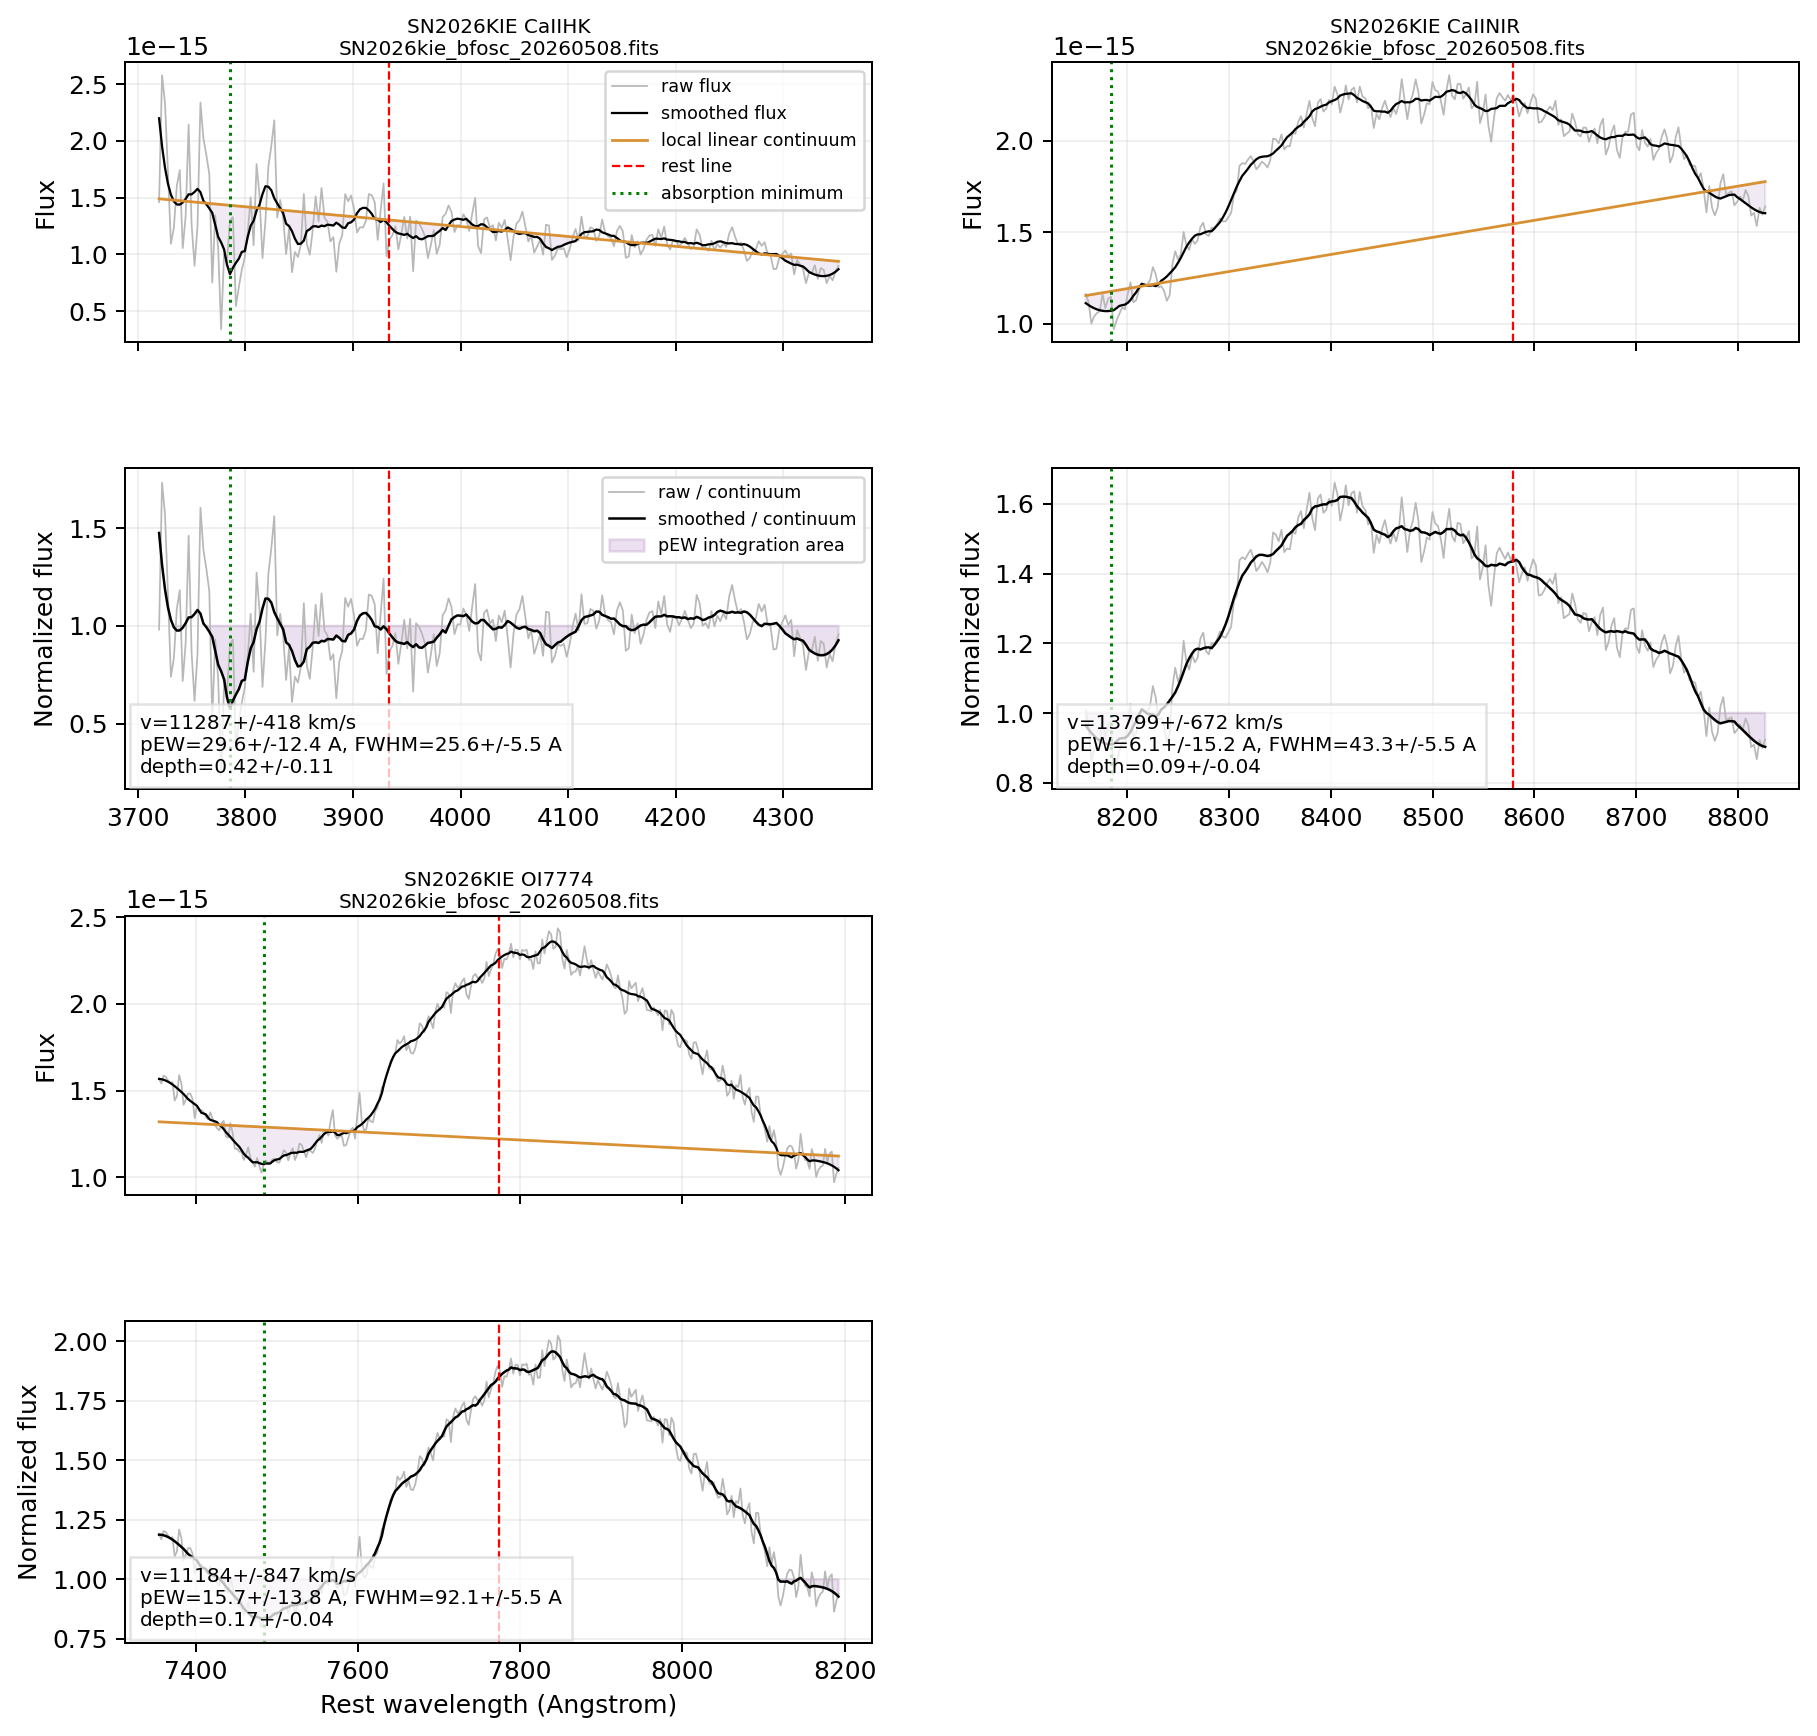
\includegraphics[width=0.96\linewidth,height=0.68\textheight,keepaspectratio]{images_zzzaurak/SN2026KIE_line_diagnostics_grid.png}
\caption{SN2026KIE 的单历元局部谱线诊断图。Ca II 与 O I 线支持 stripped-envelope 分类，但不能支持演化结论。}
\label{fig:kie-line-grid}
\end{figure}

\begin{figure}[htbp]
\centering
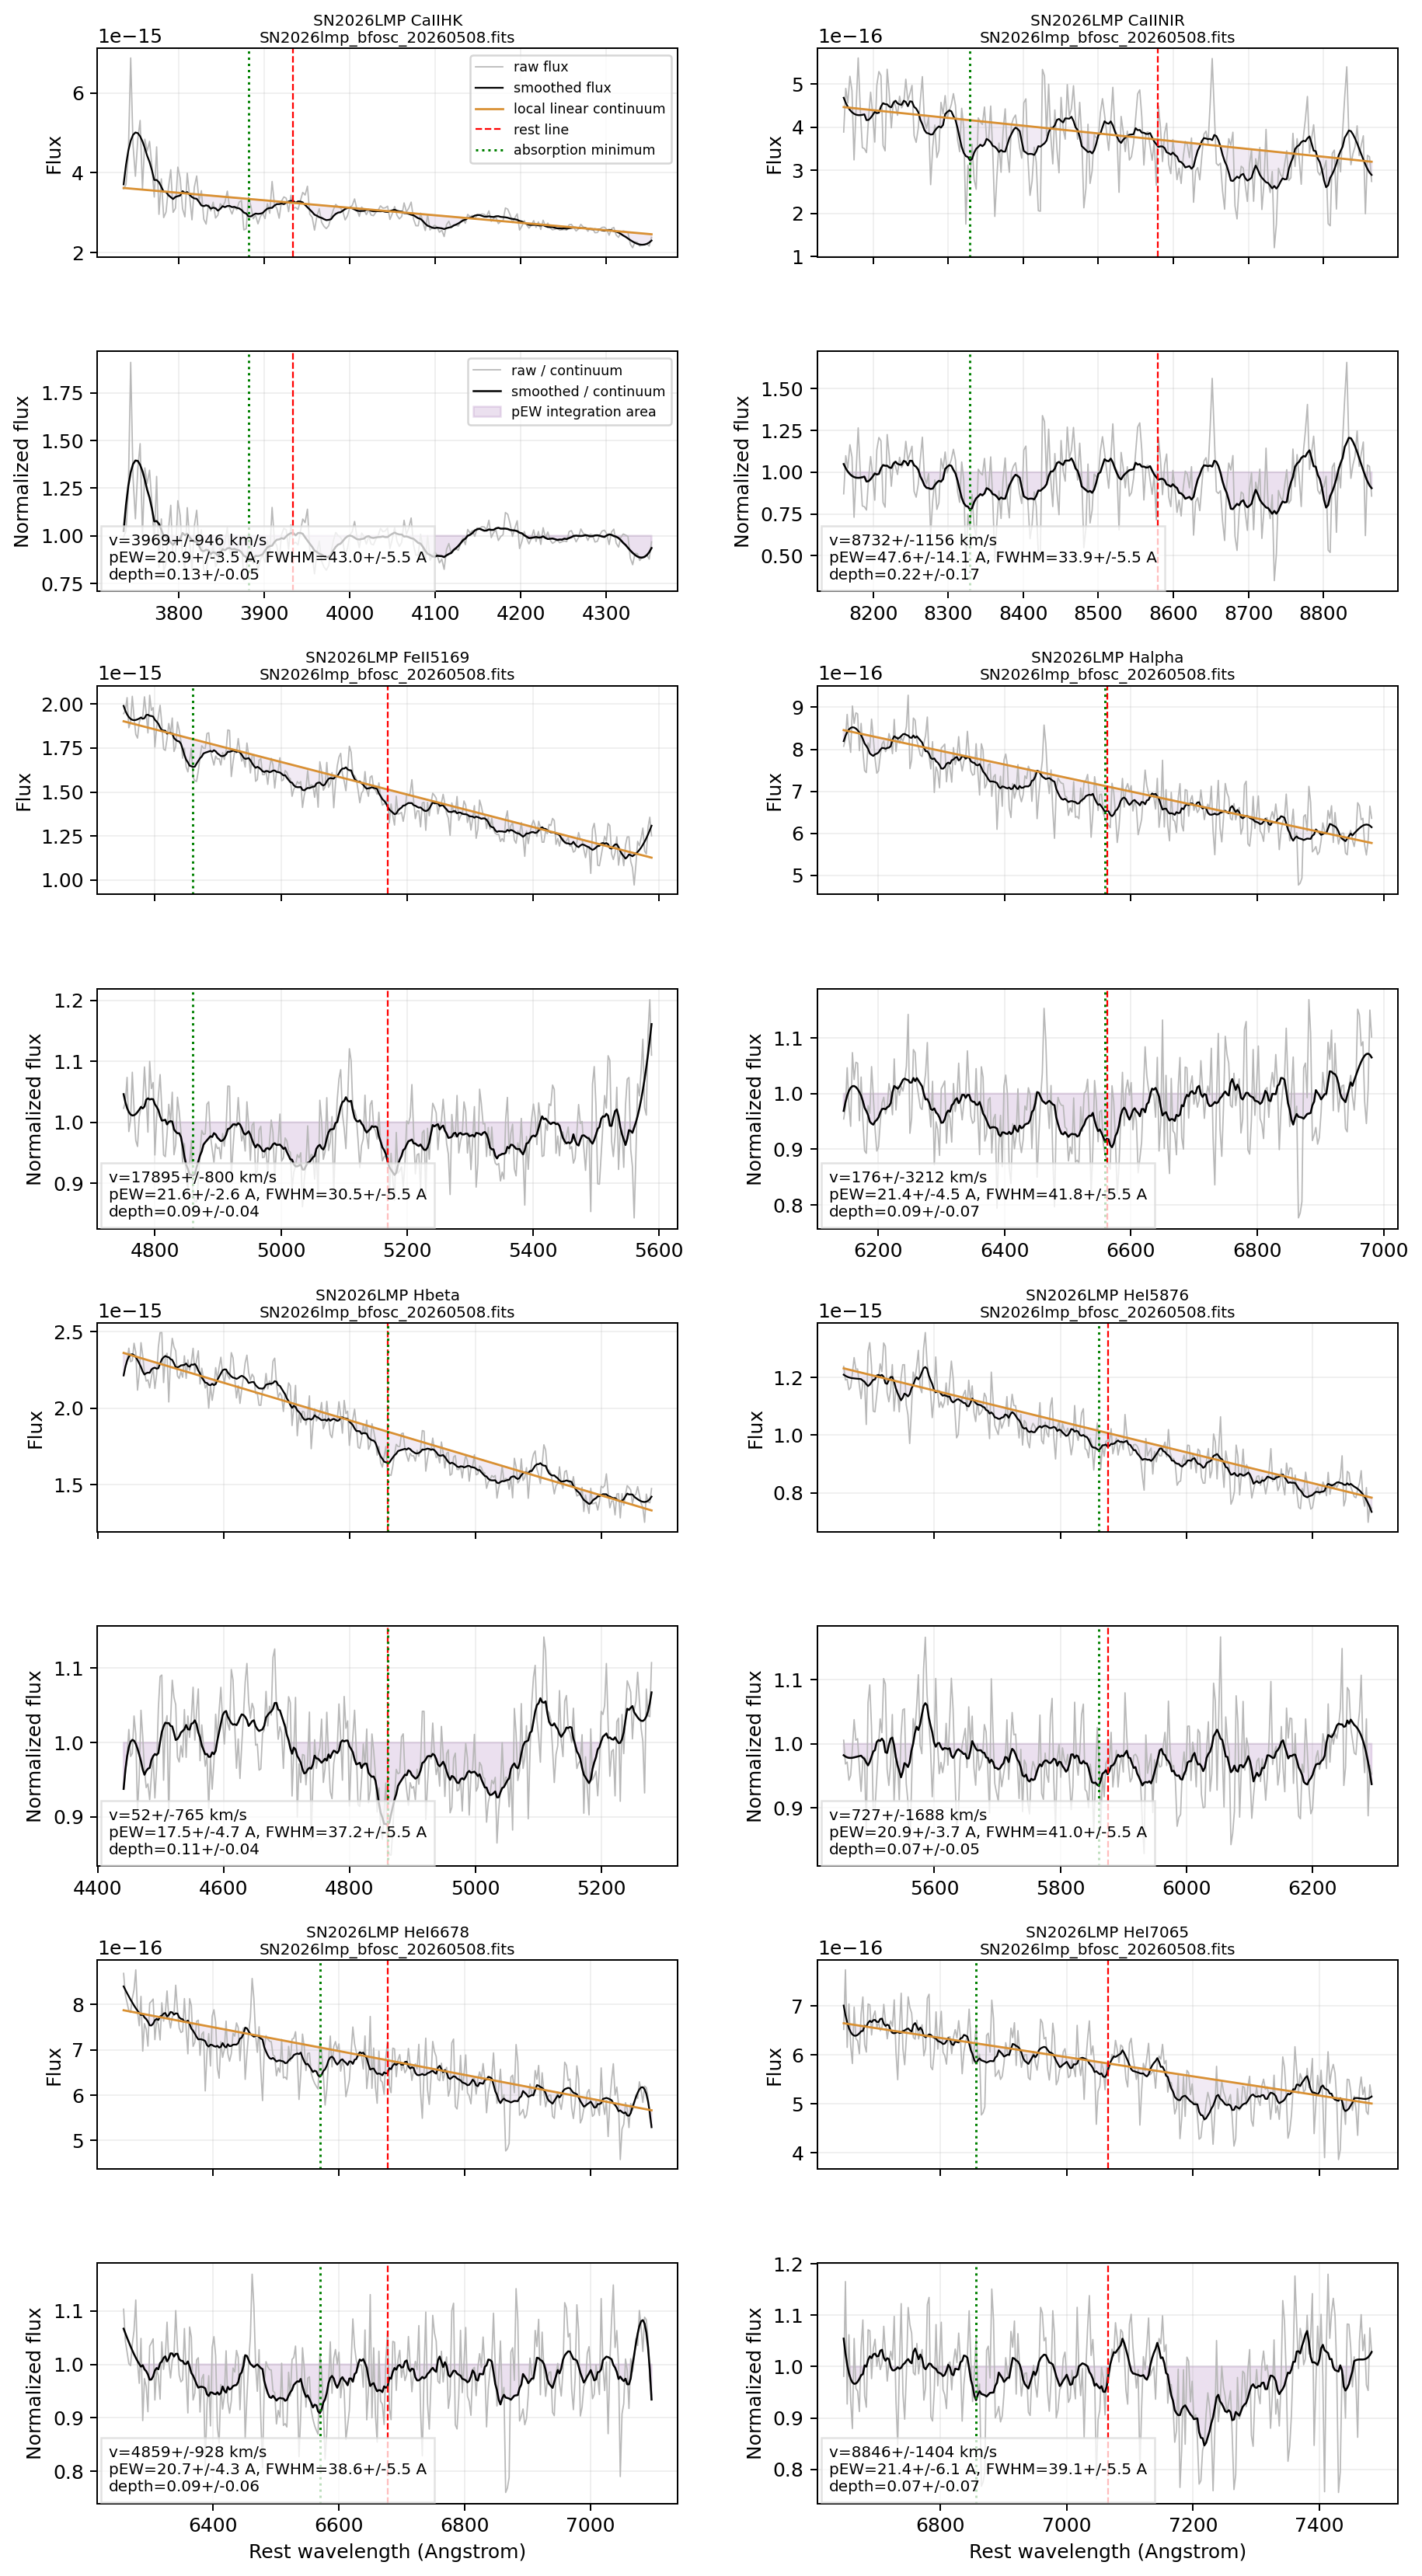
\includegraphics[width=0.96\linewidth,height=0.68\textheight,keepaspectratio]{images_zzzaurak/SN2026LMP_line_diagnostics_grid.png}
\caption{SN2026LMP 的候选线检查图。由于缺少可靠 TNS 红移，所有候选线只保留为定性检查。}
\label{fig:lmp-line-grid}
\end{figure}

\subsection{最终关键谱线测量结果}
\subsubsection{SN2026FVX}
SN2026FVX 是本样本中时间覆盖最长的 SN Ia。Si II 6355 速度从约 $1.45\times10^4~{\rm km~s^{-1}}$ 下降到约 $8.4\times10^3~{\rm km~s^{-1}}$；Ca II H\&K 也从约 $1.63\times10^4~{\rm km~s^{-1}}$ 降到约 $8.7\times10^3~{\rm km~s^{-1}}$。2026-03-26 的 Ca II H\&K 自动最低点过窄，被保留为 \code{check} 而不采用。

\begin{table}[htbp]
\centering
\caption{SN2026FVX 的 adopted 谱线测量。}
\label{tab:fvx-lines}
\begin{tabular}{r l r r r r}
\toprule
相位 & 谱线 & $v$ & pEW & FWHM & 深度 \\
天 & & km s$^{-1}$ & \AA & \AA & \\
\midrule
1.7 & CaIIHK & $16252\pm1467$ & $9.4\pm15.9$ & $45.2\pm5.5$ & 0.18 \\
20.7 & CaIIHK & $9736\pm418$ & $7.9\pm3.2$ & $36.7\pm5.5$ & 0.11 \\
51.6 & CaIIHK & $8742\pm732$ & $29.8\pm8.2$ & $47.0\pm5.5$ & 0.44 \\
1.7 & SiII6355 & $14550\pm843$ & $12.4\pm14.6$ & $60.4\pm5.5$ & 0.13 \\
8.7 & SiII6355 & $11004\pm324$ & $62.5\pm1.9$ & $126.0\pm5.5$ & 0.47 \\
20.7 & SiII6355 & $10237\pm324$ & $85.9\pm1.6$ & $128.6\pm5.5$ & 0.65 \\
51.6 & SiII6355 & $8441\pm324$ & $23.3\pm3.7$ & $58.4\pm5.5$ & 0.26 \\
\bottomrule
\end{tabular}
\end{table}

\subsubsection{SN2026JLM}
SN2026JLM 也是 SN Ia，但观测集中在发现后约 14.5--26.6 天。Si II 6355 速度保持在约 $1.1\times10^4~{\rm km~s^{-1}}$，变化不明显；Ca II H\&K 的两个采用点显示从较高到较低速度的变化，但中间历元被标为 \code{check}。

\begin{table}[htbp]
\centering
\caption{SN2026JLM 的 adopted 谱线测量。}
\label{tab:jlm-lines}
\begin{tabular}{r l r r r r}
\toprule
相位 & 谱线 & $v$ & pEW & FWHM & 深度 \\
天 & & km s$^{-1}$ & \AA & \AA & \\
\midrule
14.5 & CaIIHK & $16017\pm413$ & $12.8\pm20.2$ & $24.7\pm5.4$ & 0.24 \\
26.6 & CaIIHK & $11526\pm310$ & $22.8\pm17.2$ & $51.7\pm5.4$ & 0.32 \\
14.5 & SiII6355 & $11410\pm768$ & $74.9\pm10.1$ & $138.2\pm5.4$ & 0.57 \\
22.5 & SiII6355 & $11242\pm832$ & $88.3\pm8.0$ & $146.3\pm5.4$ & 0.59 \\
26.6 & SiII6355 & $11337\pm512$ & $77.4\pm8.7$ & $139.6\pm5.4$ & 0.55 \\
\bottomrule
\end{tabular}
\end{table}

\subsubsection{SN2026KID}
SN2026KID 为 SN II。最终只采用 Fe II 5169 作为膨胀速度量级指标。三个历元的速度约为 $0.8$--$1.1\times10^4~{\rm km~s^{-1}}$，但误差较大、线深较浅，因此不应过度解释为严格单调演化。

\begin{table}[htbp]
\centering
\caption{SN2026KID 的 adopted Fe II 5169 测量。}
\label{tab:kid-lines}
\begin{tabular}{r l r r r r}
\toprule
相位 & 谱线 & $v$ & pEW & FWHM & 深度 \\
天 & & km s$^{-1}$ & \AA & \AA & \\
\midrule
4.0 & FeII5169 & $11454\pm2714$ & $11.5\pm7.8$ & $85.7\pm5.5$ & 0.07 \\
5.0 & FeII5169 & $7723\pm1358$ & $11.5\pm8.5$ & $49.3\pm5.5$ & 0.10 \\
16.1 & FeII5169 & $8795\pm718$ & $18.7\pm7.7$ & $46.8\pm5.5$ & 0.16 \\
\bottomrule
\end{tabular}
\end{table}

\subsubsection{SN2026KIE 与 SN2026LMP}
SN2026KIE 为单历元 SN Ic。Ca II H\&K 和 O I 7774 给出约 $1.1\times10^4~{\rm km~s^{-1}}$ 的速度量级，支持 stripped-envelope SN 的解释。Ca II NIR 线深较浅且 pEW 误差大，只作为辅助。SN2026LMP 粗分类近似 SN IIb，但没有 TNS 红移；所有候选线都只作为定性检查，不采用速度、pEW 或 FWHM 作为科学结论。

\begin{table}[htbp]
\centering
\caption{SN2026KIE 的单历元 adopted 谱线测量。}
\label{tab:kie-lines}
\begin{tabular}{r l r r r r}
\toprule
相位 & 谱线 & $v$ & pEW & FWHM & 深度 \\
天 & & km s$^{-1}$ & \AA & \AA & \\
\midrule
16.3 & CaIIHK & $11287\pm418$ & $29.6\pm12.4$ & $25.6\pm5.5$ & 0.42 \\
16.3 & CaIINIR & $13799\pm672$ & $6.1\pm15.2$ & $43.3\pm5.5$ & 0.09 \\
16.3 & OI7774 & $11184\pm847$ & $15.7\pm13.8$ & $92.1\pm5.5$ & 0.17 \\
\bottomrule
\end{tabular}
\end{table}

\subsection{演化图和辅助诊断}
下面的演化图会同时显示 \code{adopt} 和 \code{check} 行，用来保留人工复核痕迹；定量结论只引用前面表中的 \code{adopt} 测量。图中透明度较低或孤立的 \code{check} 点，尤其是 SN2026LMP 的缺红移候选线，只能作为诊断参考，不进入速度、pEW 或 FWHM 结论。误差棒缺失或很大时，表示最低点定位、局部噪声或连续谱窗口带来的不确定性较大。

\begin{figure}[htbp]
\centering
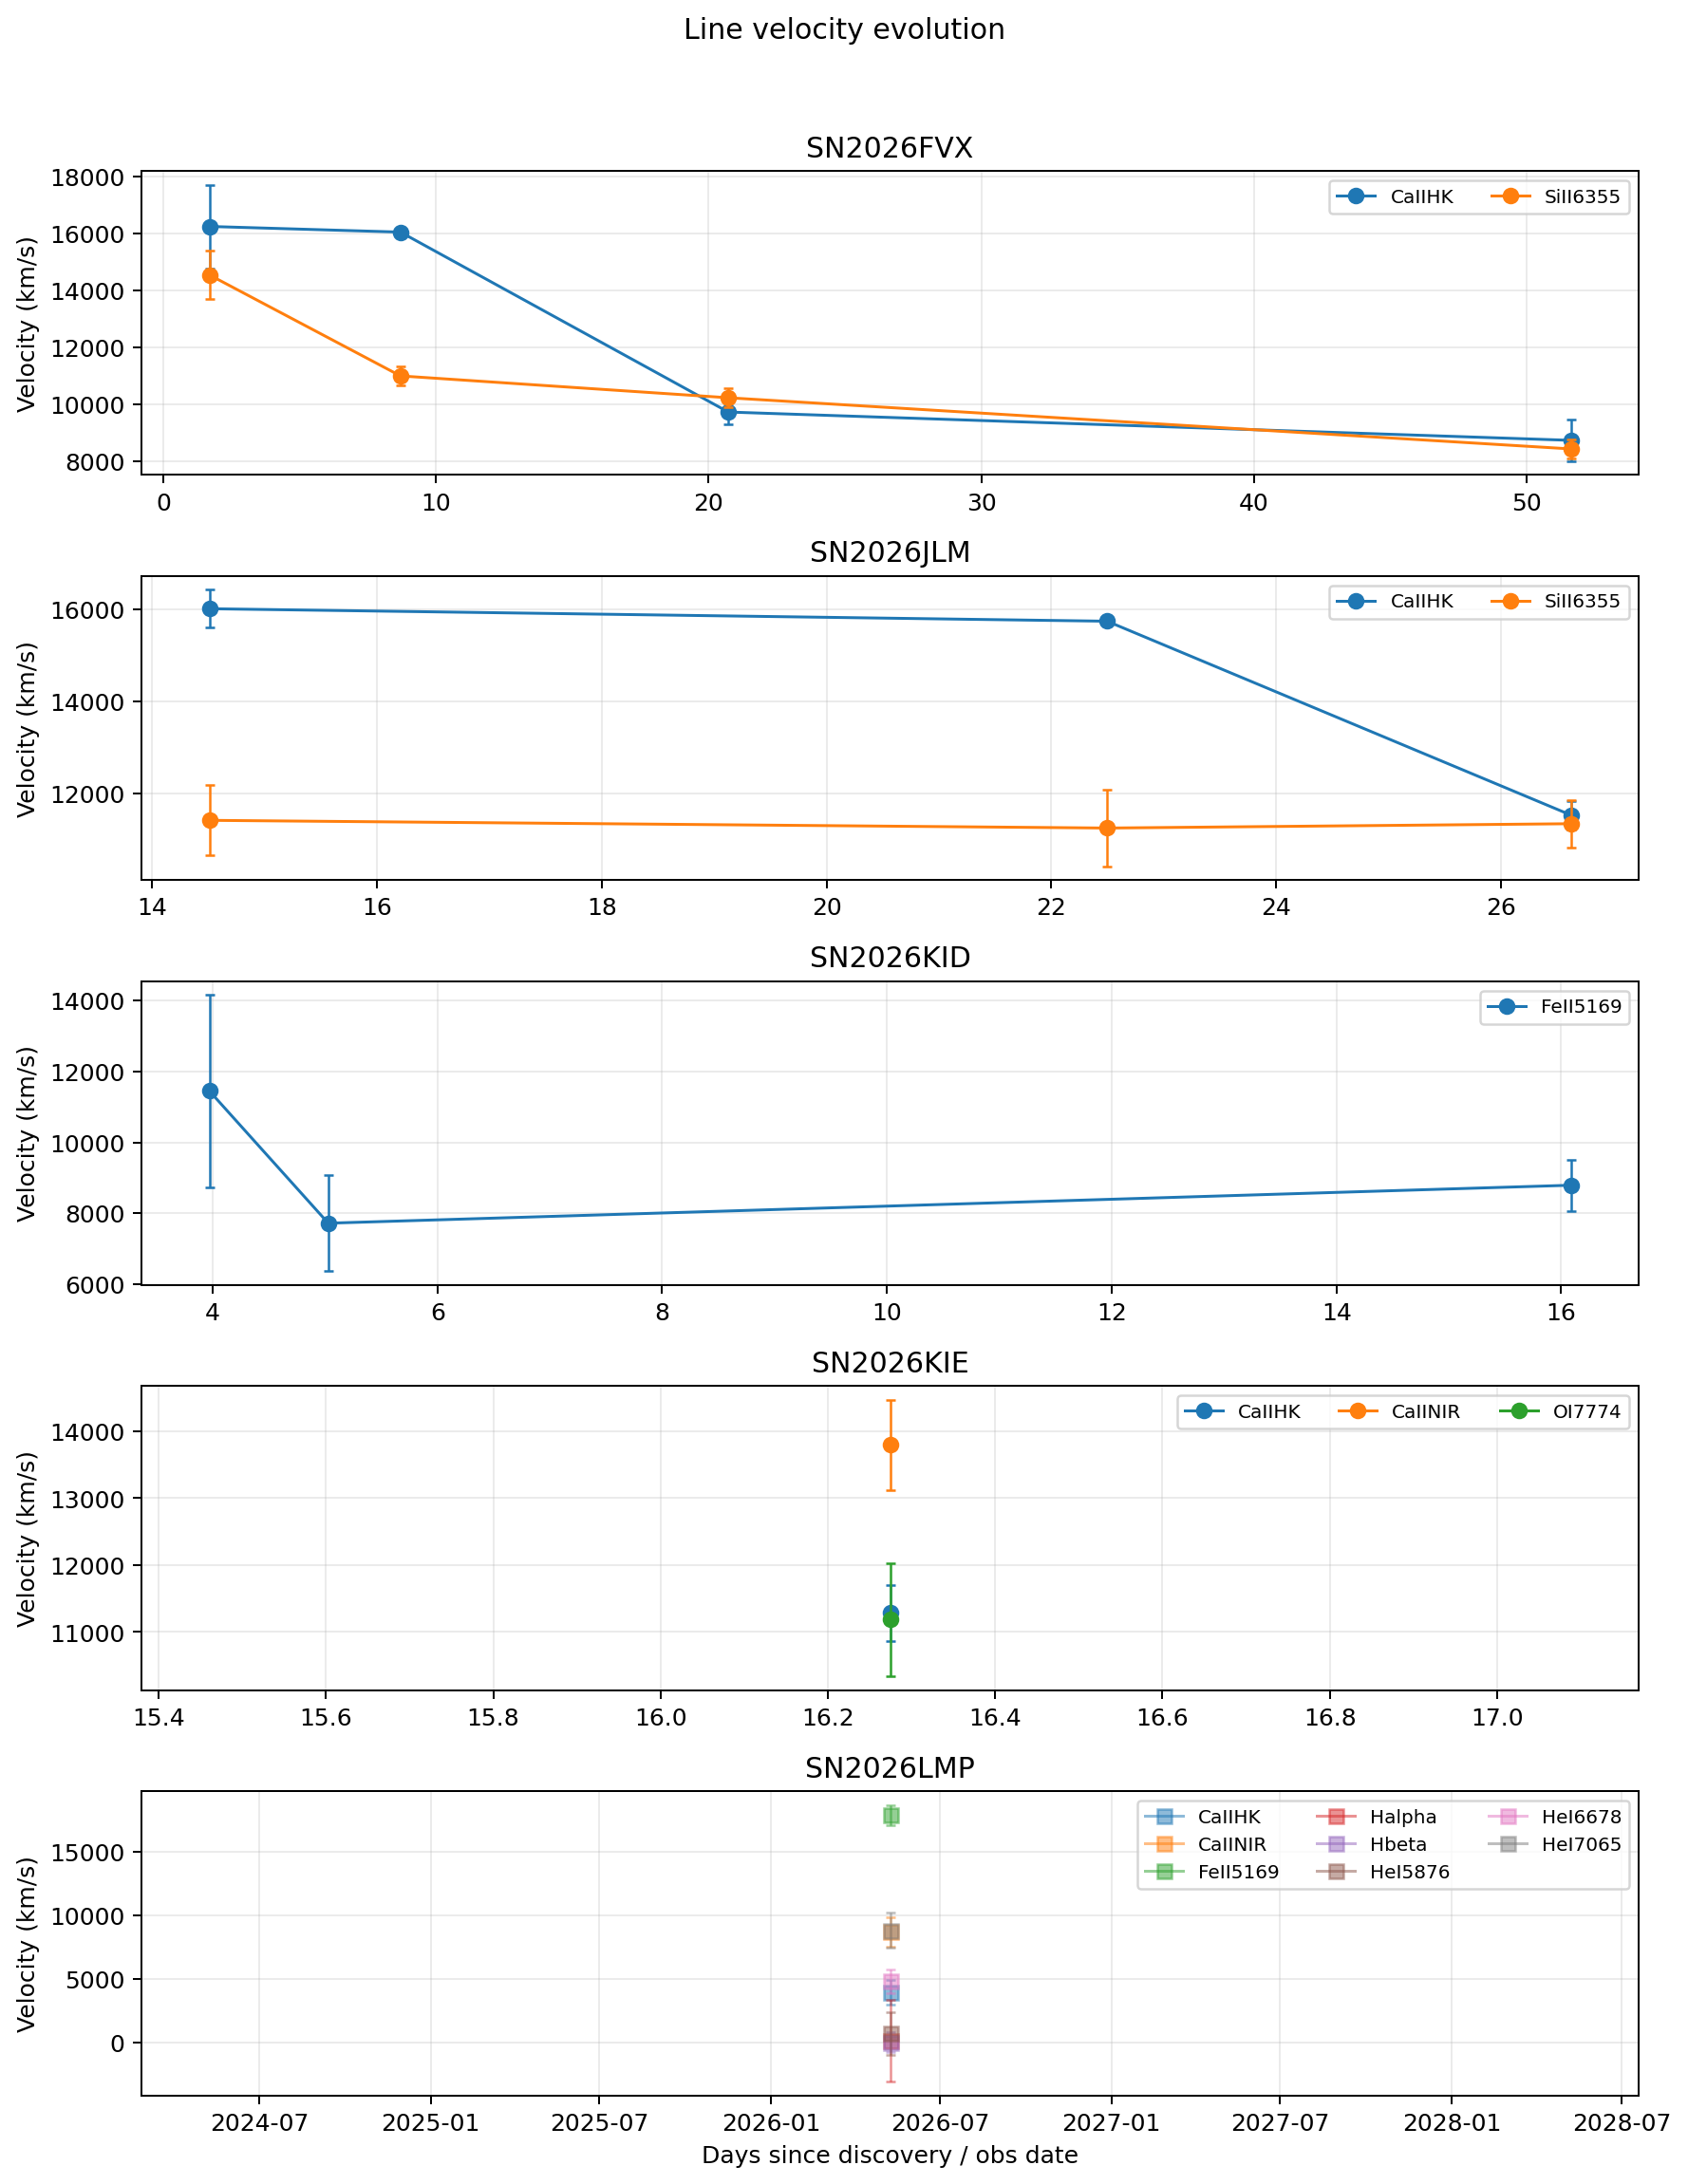
\includegraphics[width=0.95\linewidth]{images_zzzaurak/final5_line_velocity_evolution.png}
\caption{谱线速度随距发现日天数的演化。SN2026FVX 的 Si II 6355 和 Ca II H\&K 速度下降最清楚；SN2026JLM 的 Si II 6355 在较短相位范围内较稳定。}
\label{fig:velocity-evolution}
\end{figure}

\begin{figure}[htbp]
\centering
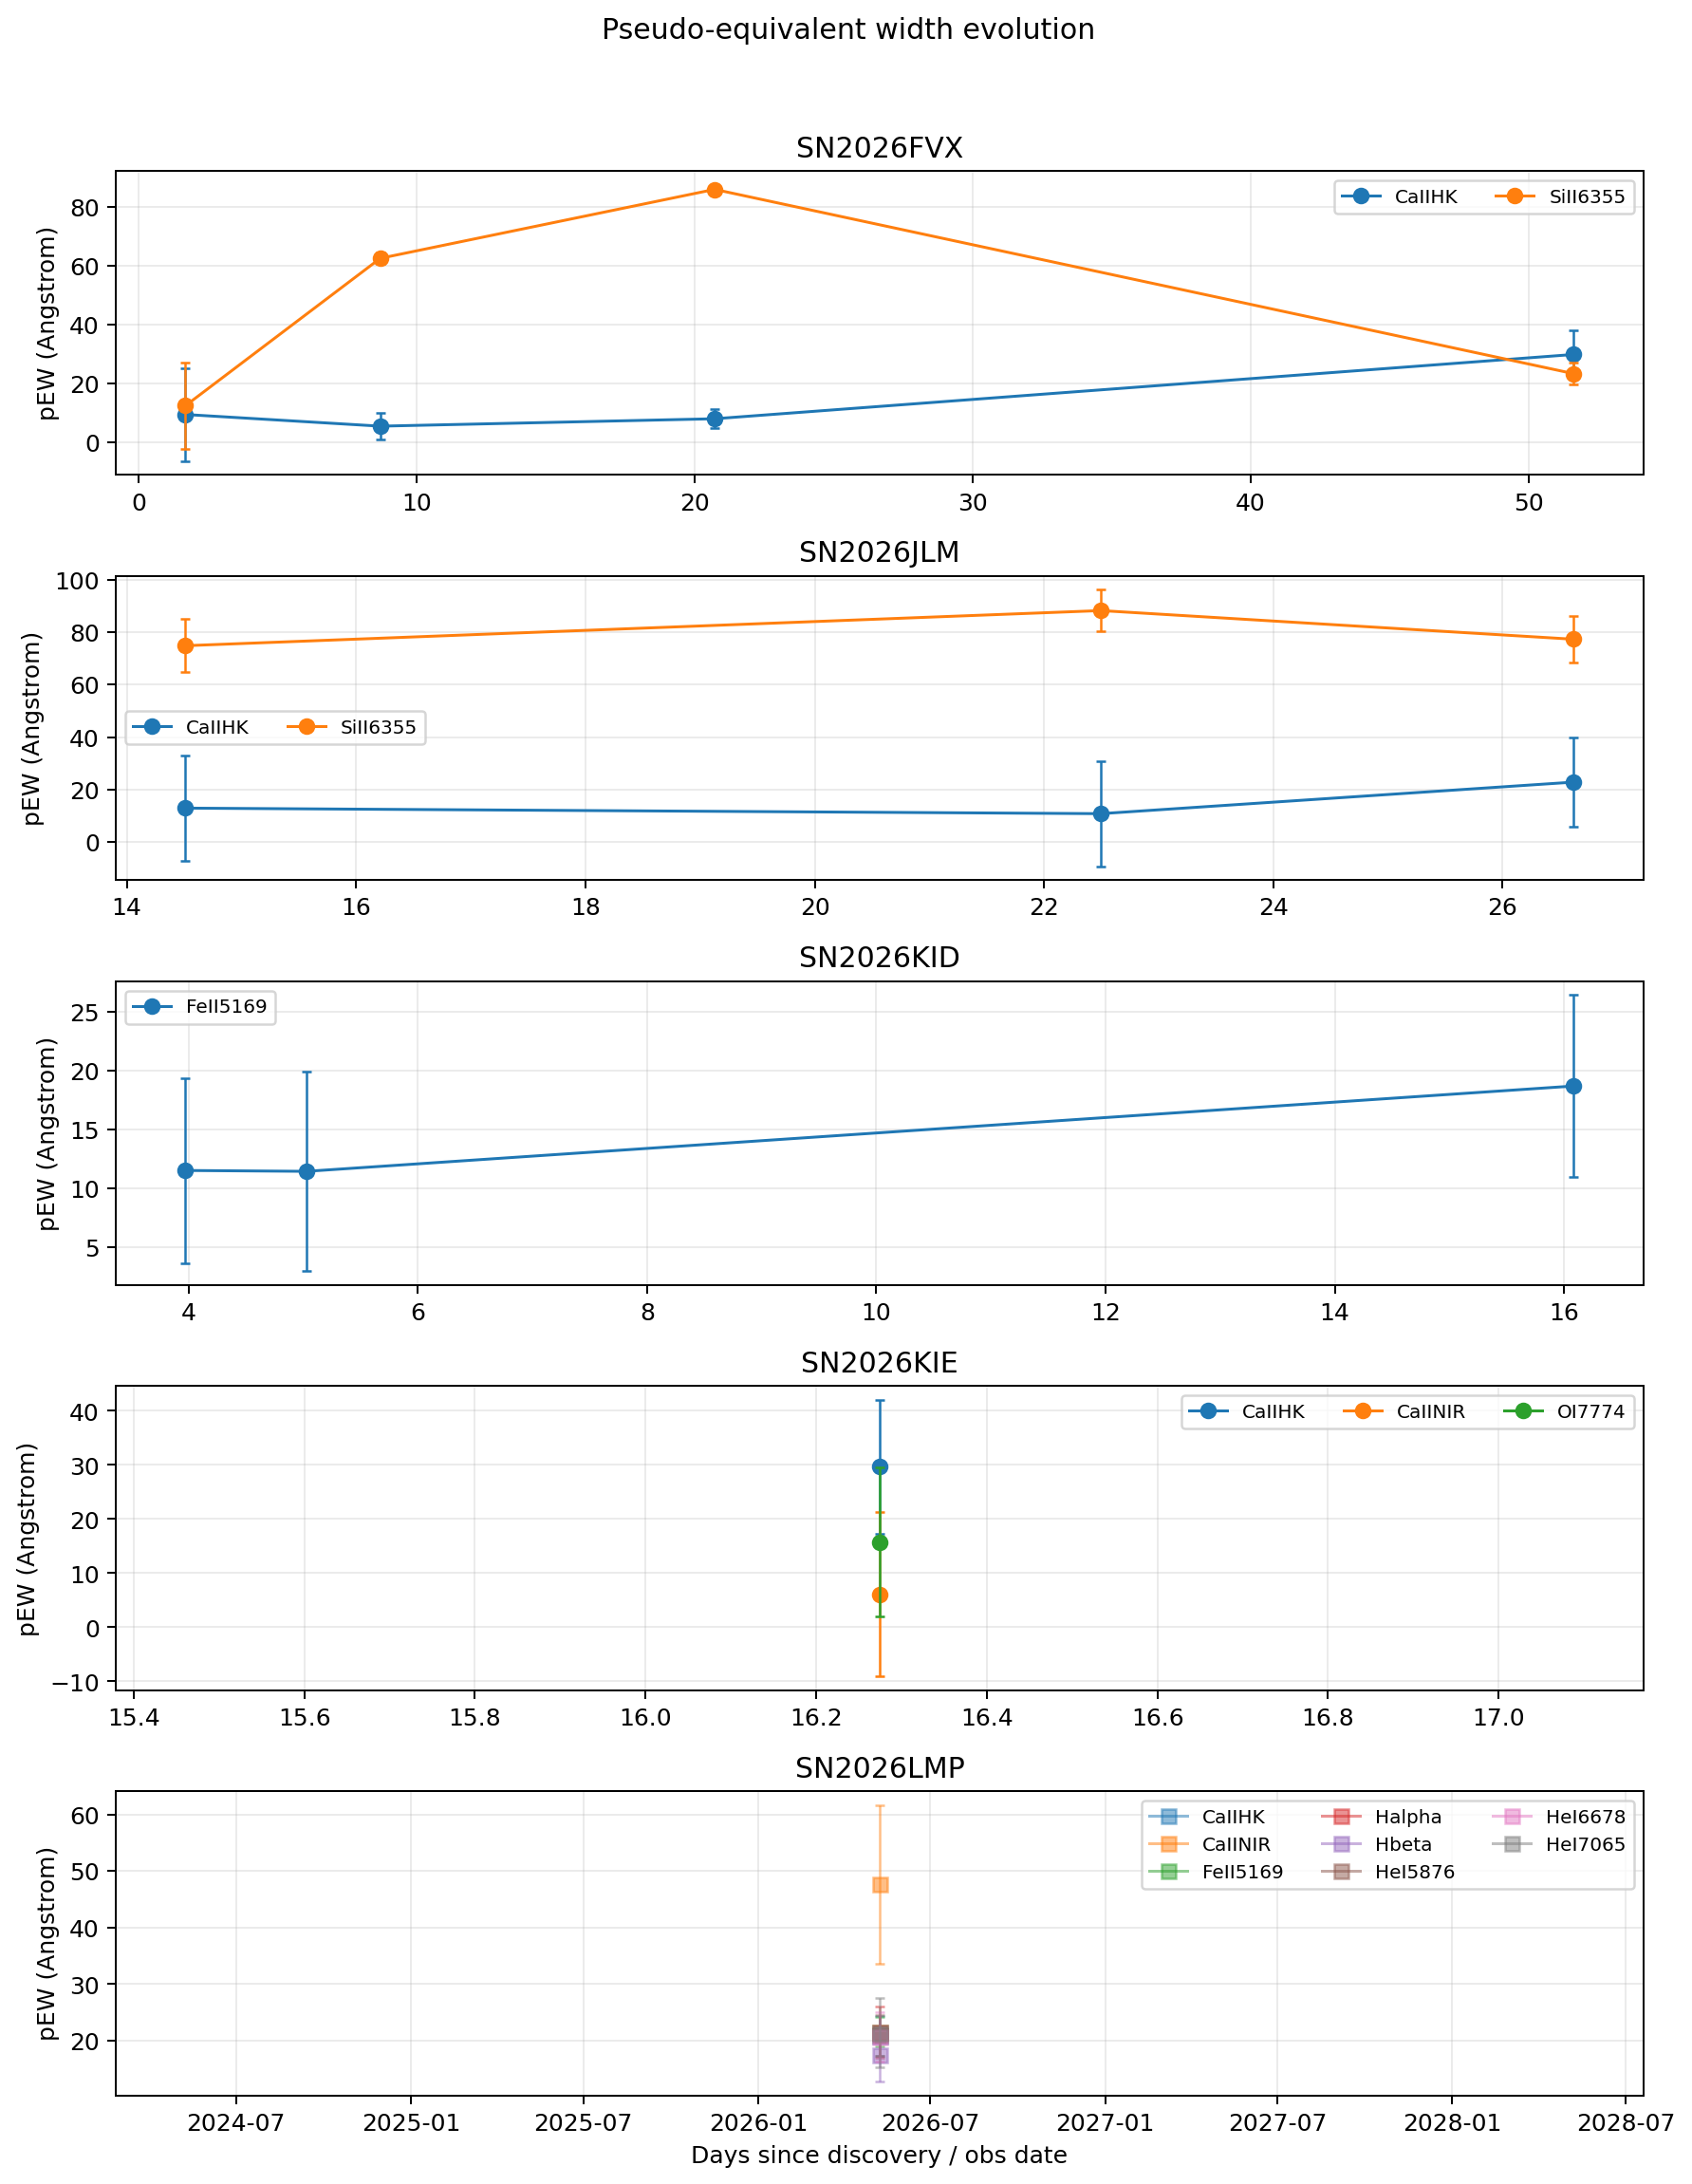
\includegraphics[width=0.95\linewidth]{images_zzzaurak/final5_pew_evolution.png}
\caption{关键谱线 pEW 的演化。pEW 对局部连续谱和线混合更敏感，因此弱线或误差较大的点只作辅助。}
\label{fig:pew-evolution}
\end{figure}

\begin{figure}[htbp]
\centering
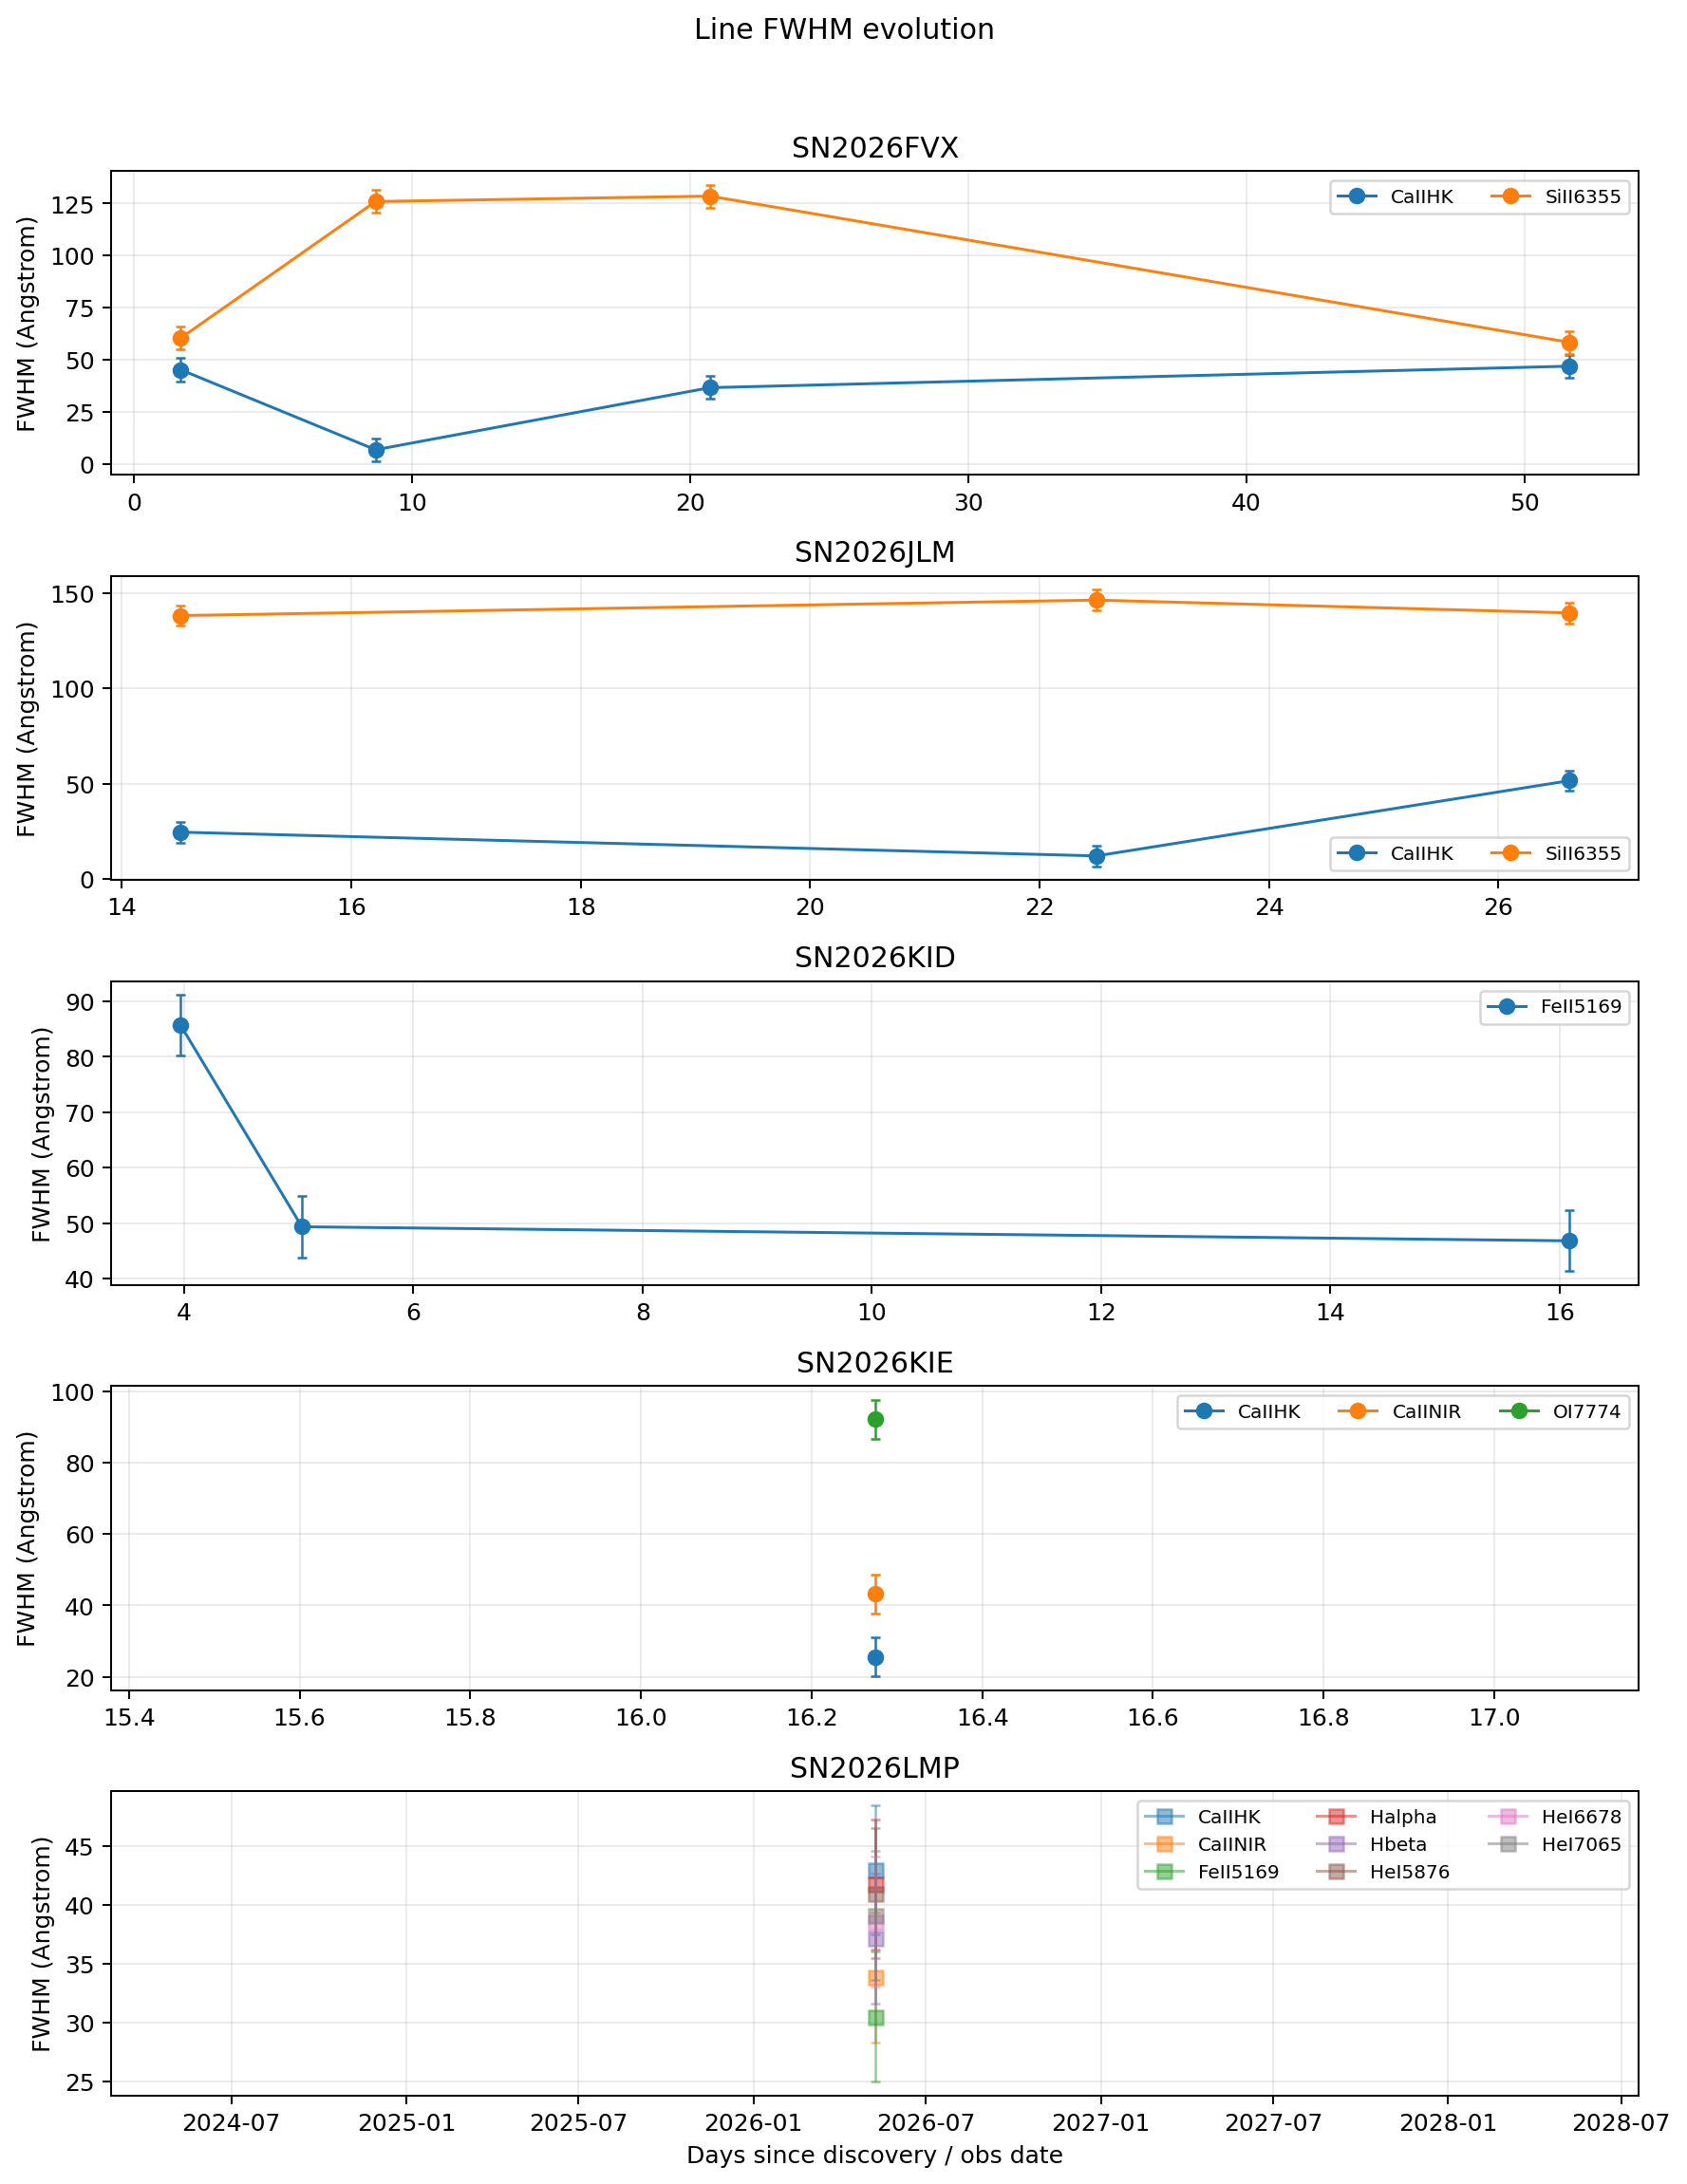
\includegraphics[width=0.95\linewidth]{images_zzzaurak/final5_fwhm_evolution.png}
\caption{非参数半深度 FWHM 演化图。该宽度由最低点两侧半深度交点给出。}
\label{fig:fwhm-evolution}
\end{figure}

\begin{figure}[htbp]
\centering
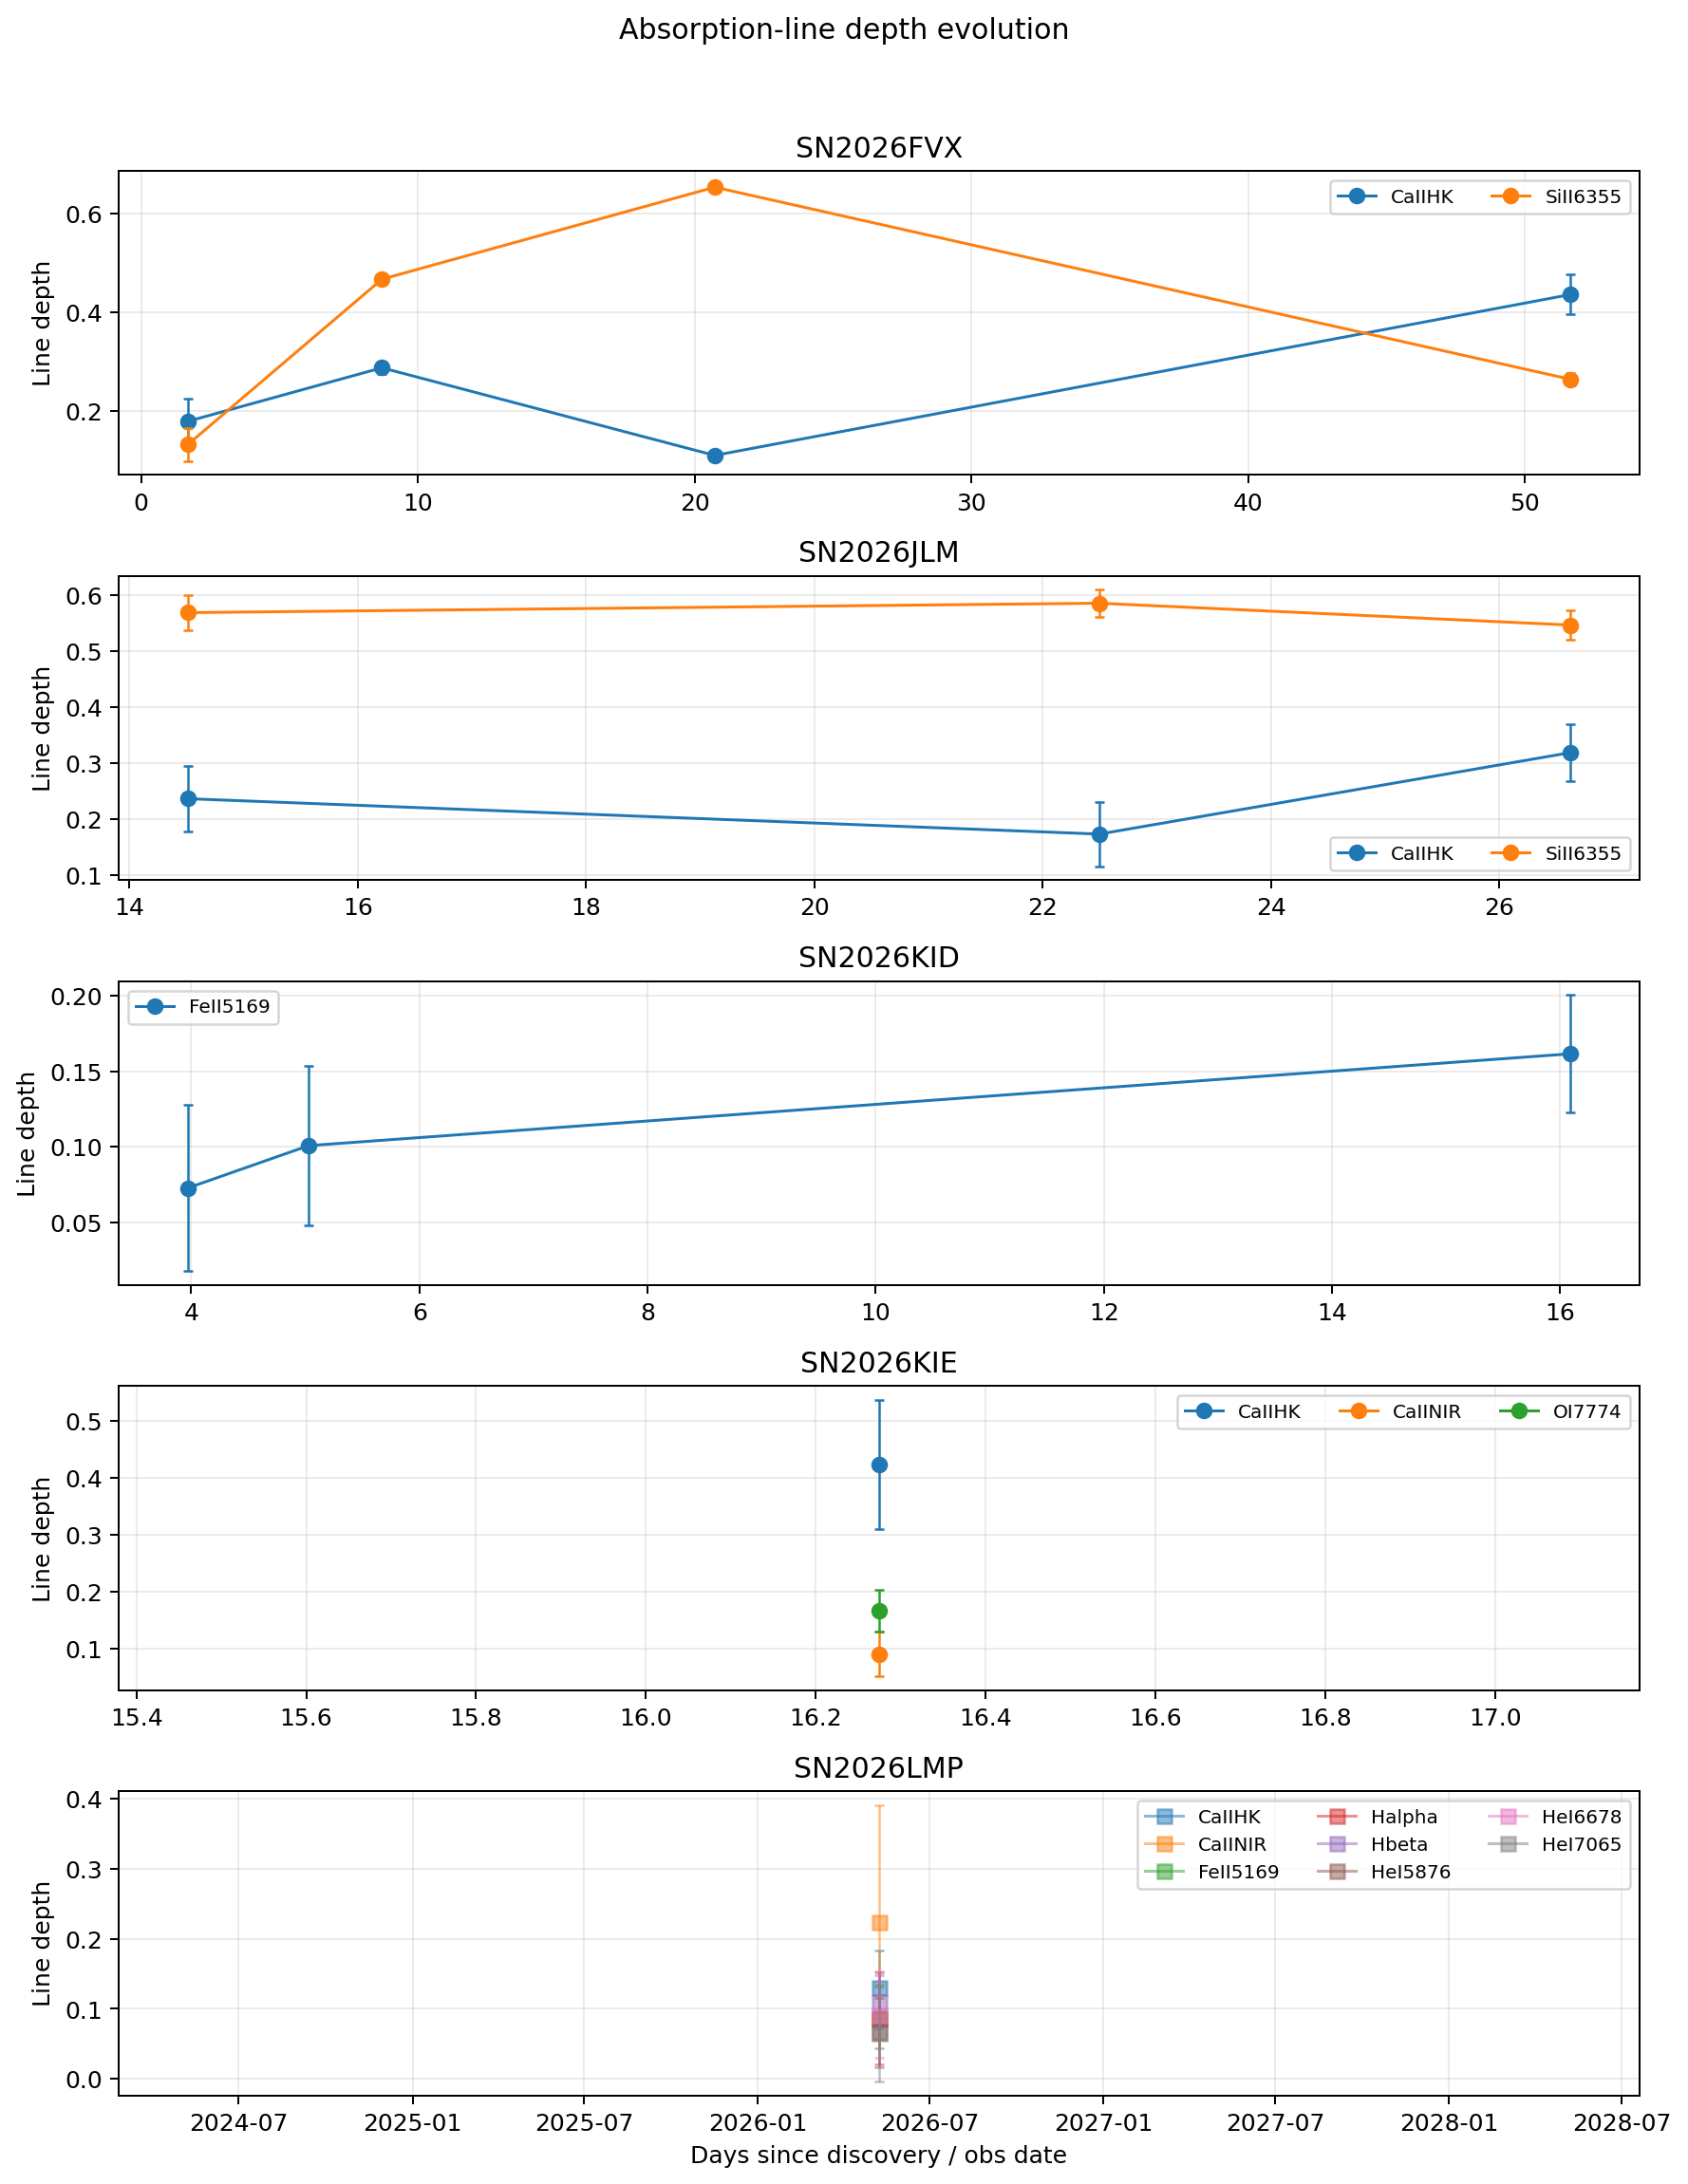
\includegraphics[width=0.95\linewidth]{images_zzzaurak/final5_line_depth_evolution.png}
\caption{吸收线深度演化图。线深浅且误差大的点不适合做强物理解释。}
\label{fig:depth-evolution}
\end{figure}

黑体颜色温度只作为连续谱形状代理。这张演化图统一使用 \code{phase\_days} 作为横坐标；SN2026LMP 缺少距发现日相位，因此不画入该演化图，只保留在 CSV 和单谱拟合检查中。SN2026KID、SN2026KIE 和 SN2026LMP 的蓝端形状或红移条件不够可靠，因此温度不作为主要科学结论。

\begin{figure}[htbp]
\centering
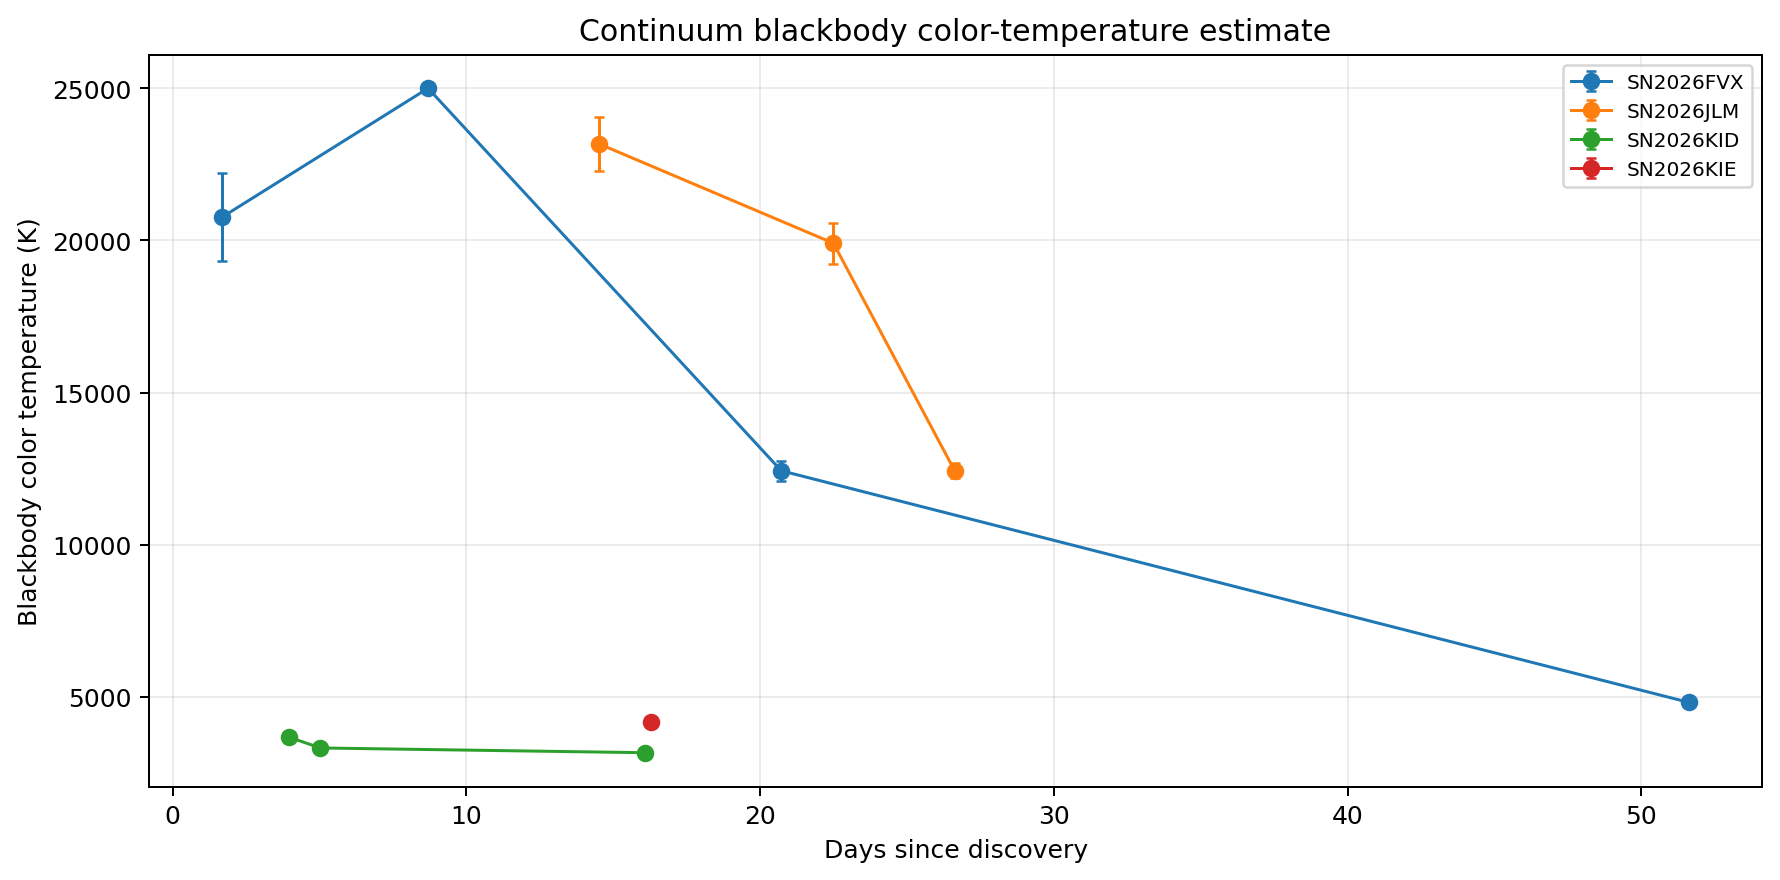
\includegraphics[width=0.95\linewidth]{images_zzzaurak/final5_blackbody_temperature.png}
\caption{连续谱黑体颜色温度代理。该图用于描述连续谱形状变化，不是完整辐射输运温度测量。}
\label{fig:blackbody-temperature}
\end{figure}

\subsection{TARDIS 辐射输运模拟作为定性辅助分析}
除了前面的经验谱线测量，我还使用 TARDIS 做了一组一维 Monte Carlo 辐射输运模拟，用来检查主要谱线识别和速度范围是否合理。TARDIS 在本项目中只是辅助分析，不是主证据链，也不是严格的物理参数反演。由于本项目每颗超新星的光谱历元较少、光变曲线约束不足，模型中的 luminosity、爆炸后时间、速度边界、密度结构和丰度 preset 都是为了让合成光谱在主要谱线位置和大尺度谱形上接近观测，而不能直接解释为真实的抛射物质量、元素丰度或爆炸能量。

本次没有对每个历元分别建模，而是每颗有可靠红移和分类的超新星选取一条代表性早期光谱。四个 TARDIS 目标分别为 SN2026FVX、SN2026JLM、SN2026KID 和 SN2026KIE；SN2026LMP 因缺少可靠 TNS 红移，没有做 TARDIS 定量比较。观测谱仍按前文同样的方式除以 $(1+z)$ 转到静止系。模拟谱和观测谱都经过相同的平滑和 pseudo-continuum normalization 后比较，因此图中重点是谱线位置和相对形状，而不是绝对流量。

TARDIS 候选参数主要包括总 luminosity、爆炸后时间、速度范围、密度 profile、丰度 preset 和 plasma 设定。Ia 目标使用 \code{branch85\_w7} 这类 W7-like 密度结构；II 和 Ibc 目标使用 \code{exponential} 或 \code{power\_law} 这类简化密度结构。丰度不是逐层拟合，而是少量 uniform preset，例如 \code{ia\_standard}、\code{ia\_si\_rich}、\code{ii\_h\_rich} 和 \code{ib\_he\_rich}。我还测试了 TARDIS 包自带的 Ia CSVY 分层模型资源，以及更接近文献光球近似的 \code{nebular + dilute-lte + macroatom} plasma preset。实际检查发现，这些更复杂或更接近文献设定的配置并不自动给出更好的拟合；最终采用仍以 final-packet 复跑和目视检查为准。

评分函数不是比较原始 flux，而是在全局重叠波段和几个诊断谱线窗口中比较归一化谱形。总分由 broad RMSE、谱线窗口 RMSE、相关系数惩罚和吸收谷位置偏差组成，分数越低表示在当前归一化和线窗定义下越接近。Ia 目标重点比较 Ca II H\&K、Si II 5972、Si II 6355 和 Ca II NIR；SN II 重点比较 H$\beta$、Fe II 5169 和 H$\alpha$；Ibc 重点比较 Ca II H\&K、Fe II 5169、O I 7774 和 Ca II NIR。

\begin{table}[htbp]
\centering
\caption{最终采用的 TARDIS 定性比较参数。分数只用于同一套归一化和线窗下的模型筛选，不应解释为真实物理优劣。}
\label{tab:tardis-adopted}
\resizebox{\linewidth}{!}{%
\begin{tabular}{l l r r r l l l}
\toprule
目标 & 候选 & 分数 & $\log L/L_\odot$ & 时间（天） & 速度范围（km s$^{-1}$） & 密度 & 丰度 preset \\
\midrule
SN2026FVX & \code{SN2026FVX\_c000} & 1.037 & 9.40 & 25.7 & 4374--13538 & \code{branch85\_w7} & \code{ia\_standard} \\
SN2026JLM & \code{SN2026JLM\_c001} & 1.753 & 9.40 & 32.5 & 5019--15534 & \code{branch85\_w7} & \code{ia\_si\_rich} \\
SN2026KID & \code{SN2026KID\_c002} & 1.136 & 8.80 & 25.0 & 5764--12488 & \code{exponential} & \code{ii\_h\_rich} \\
SN2026KIE & \code{SN2026KIE\_c000} & 1.287 & 9.00 & 31.3 & 8055--17452 & \code{power\_law} & \code{ib\_he\_rich} \\
\bottomrule
\end{tabular}}
\end{table}

从单目标结果看，SN2026FVX 的 Ia 模型在 Si II 6355 主吸收附近与观测谱基本对齐，能支持 Ia 谱线识别；蓝端 Ca II H\&K 和 Ca II NIR 仍有明显强度差异。SN2026JLM 的 Si II 6355 也有对应结构，但模拟吸收中心略偏蓝，Ca II NIR 偏深，因此只作为定性支持。SN2026KID 是四个目标中 TARDIS 对比最稳定的一个，H$\alpha$ 区域的 P-Cygni 形状和速度范围与观测有较好对应，可作为 Type II 光谱解释的 sanity check。SN2026KIE 的 Ibc 模型能部分复现 O I 7774 和 Ca II NIR 区域；最新 adopted 模型将速度范围略向高速度移动后，6200--6400~\AA\ 附近的过深吸收稍有缓解，但 Ca II NIR 仍偏深。

\begin{figure}[htbp]
\centering
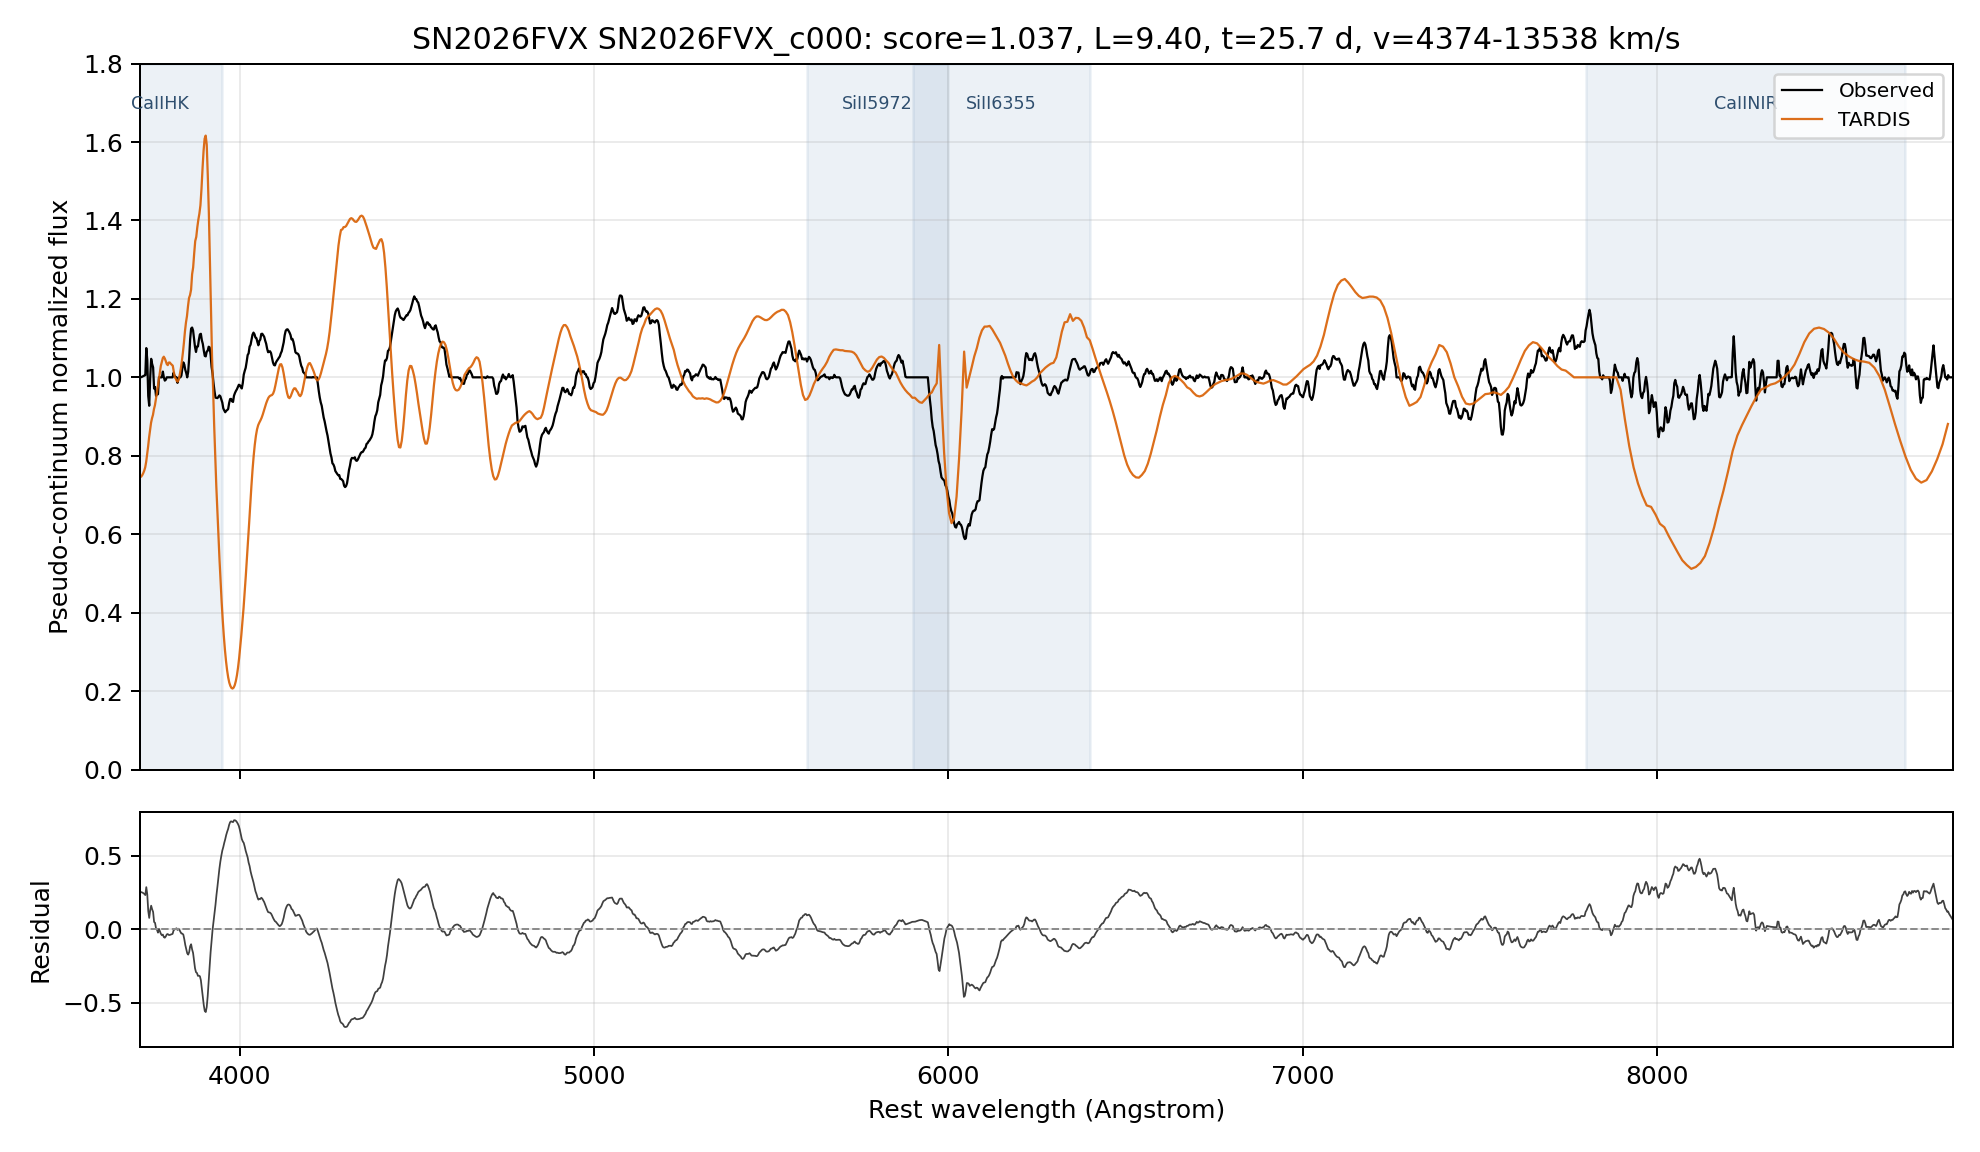
\includegraphics[width=0.95\linewidth]{images_zzzaurak/tardis_comparison_SN2026FVX.png}
\caption{SN2026FVX 的 TARDIS 定性比较。模型主要用于检查 Si II 6355 与 Ca II 区域的谱线位置。}
\label{fig:tardis-fvx}
\end{figure}

\begin{figure}[htbp]
\centering
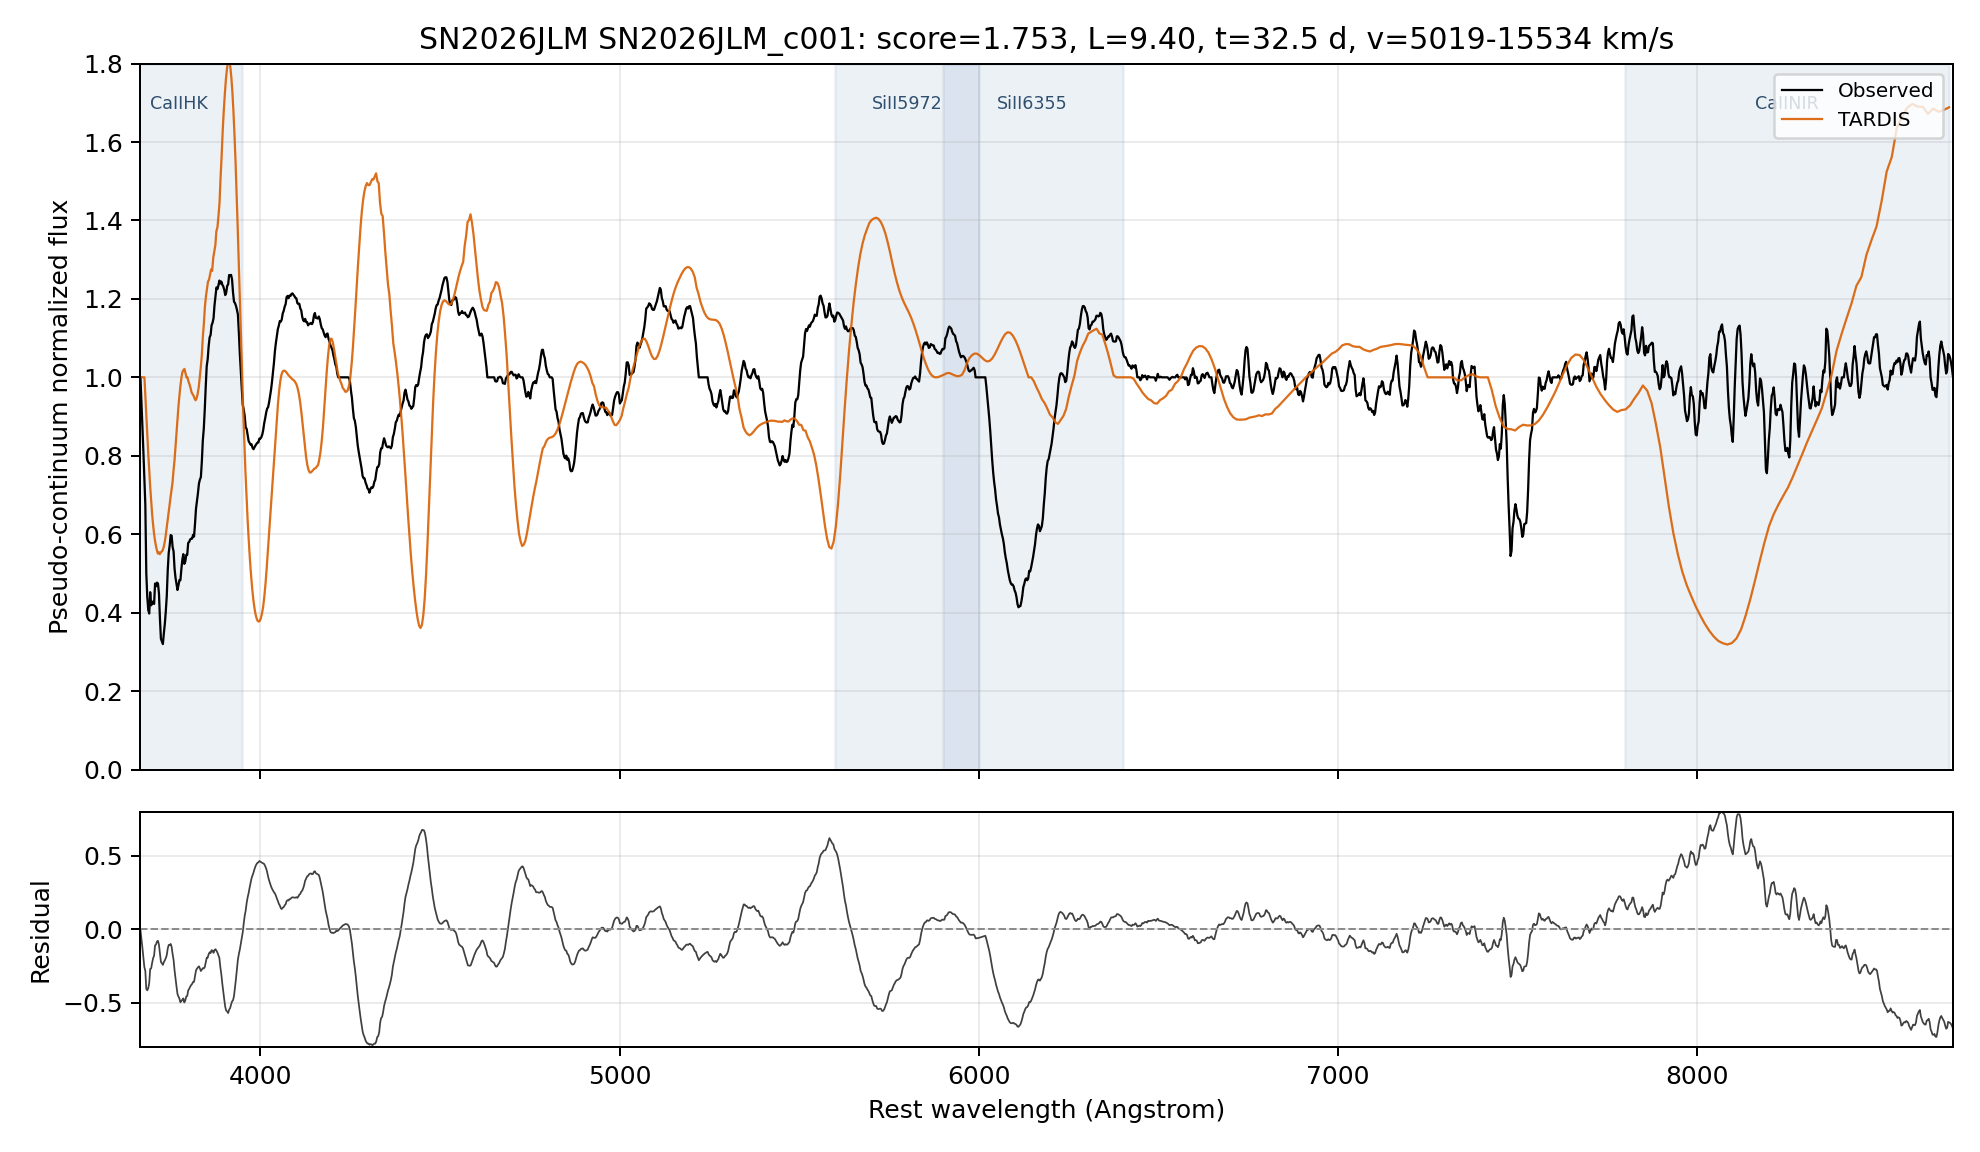
\includegraphics[width=0.95\linewidth]{images_zzzaurak/tardis_comparison_SN2026JLM.png}
\caption{SN2026JLM 的 TARDIS 定性比较。该图支持 Ia 谱线识别，但不提供丰度或爆炸参数反演。}
\label{fig:tardis-jlm}
\end{figure}

\begin{figure}[htbp]
\centering
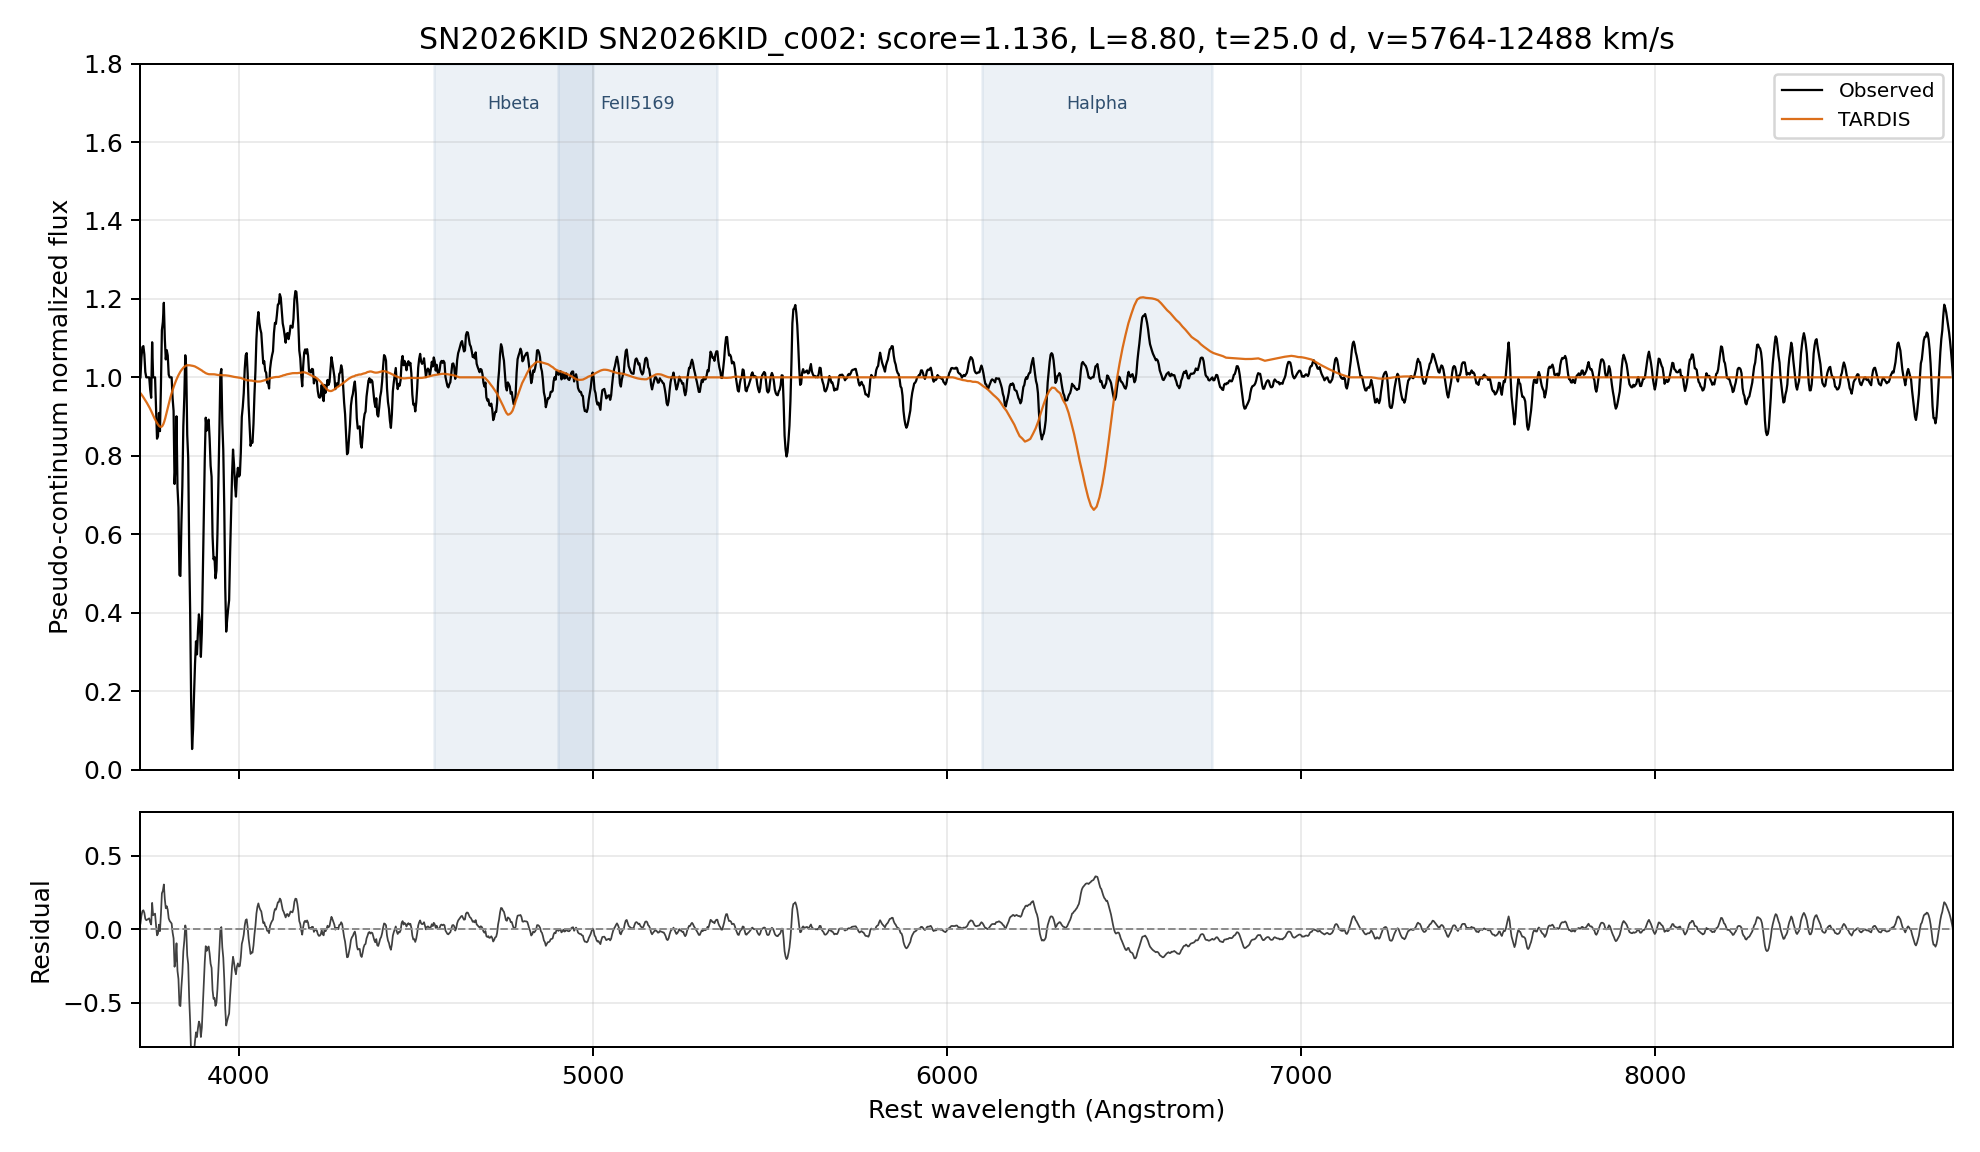
\includegraphics[width=0.95\linewidth]{images_zzzaurak/tardis_comparison_SN2026KID.png}
\caption{SN2026KID 的 TARDIS 定性比较。H$\alpha$ 的 P-Cygni 形状与观测有较好对应，是 Type II 解释的辅助证据。}
\label{fig:tardis-kid}
\end{figure}

\begin{figure}[htbp]
\centering
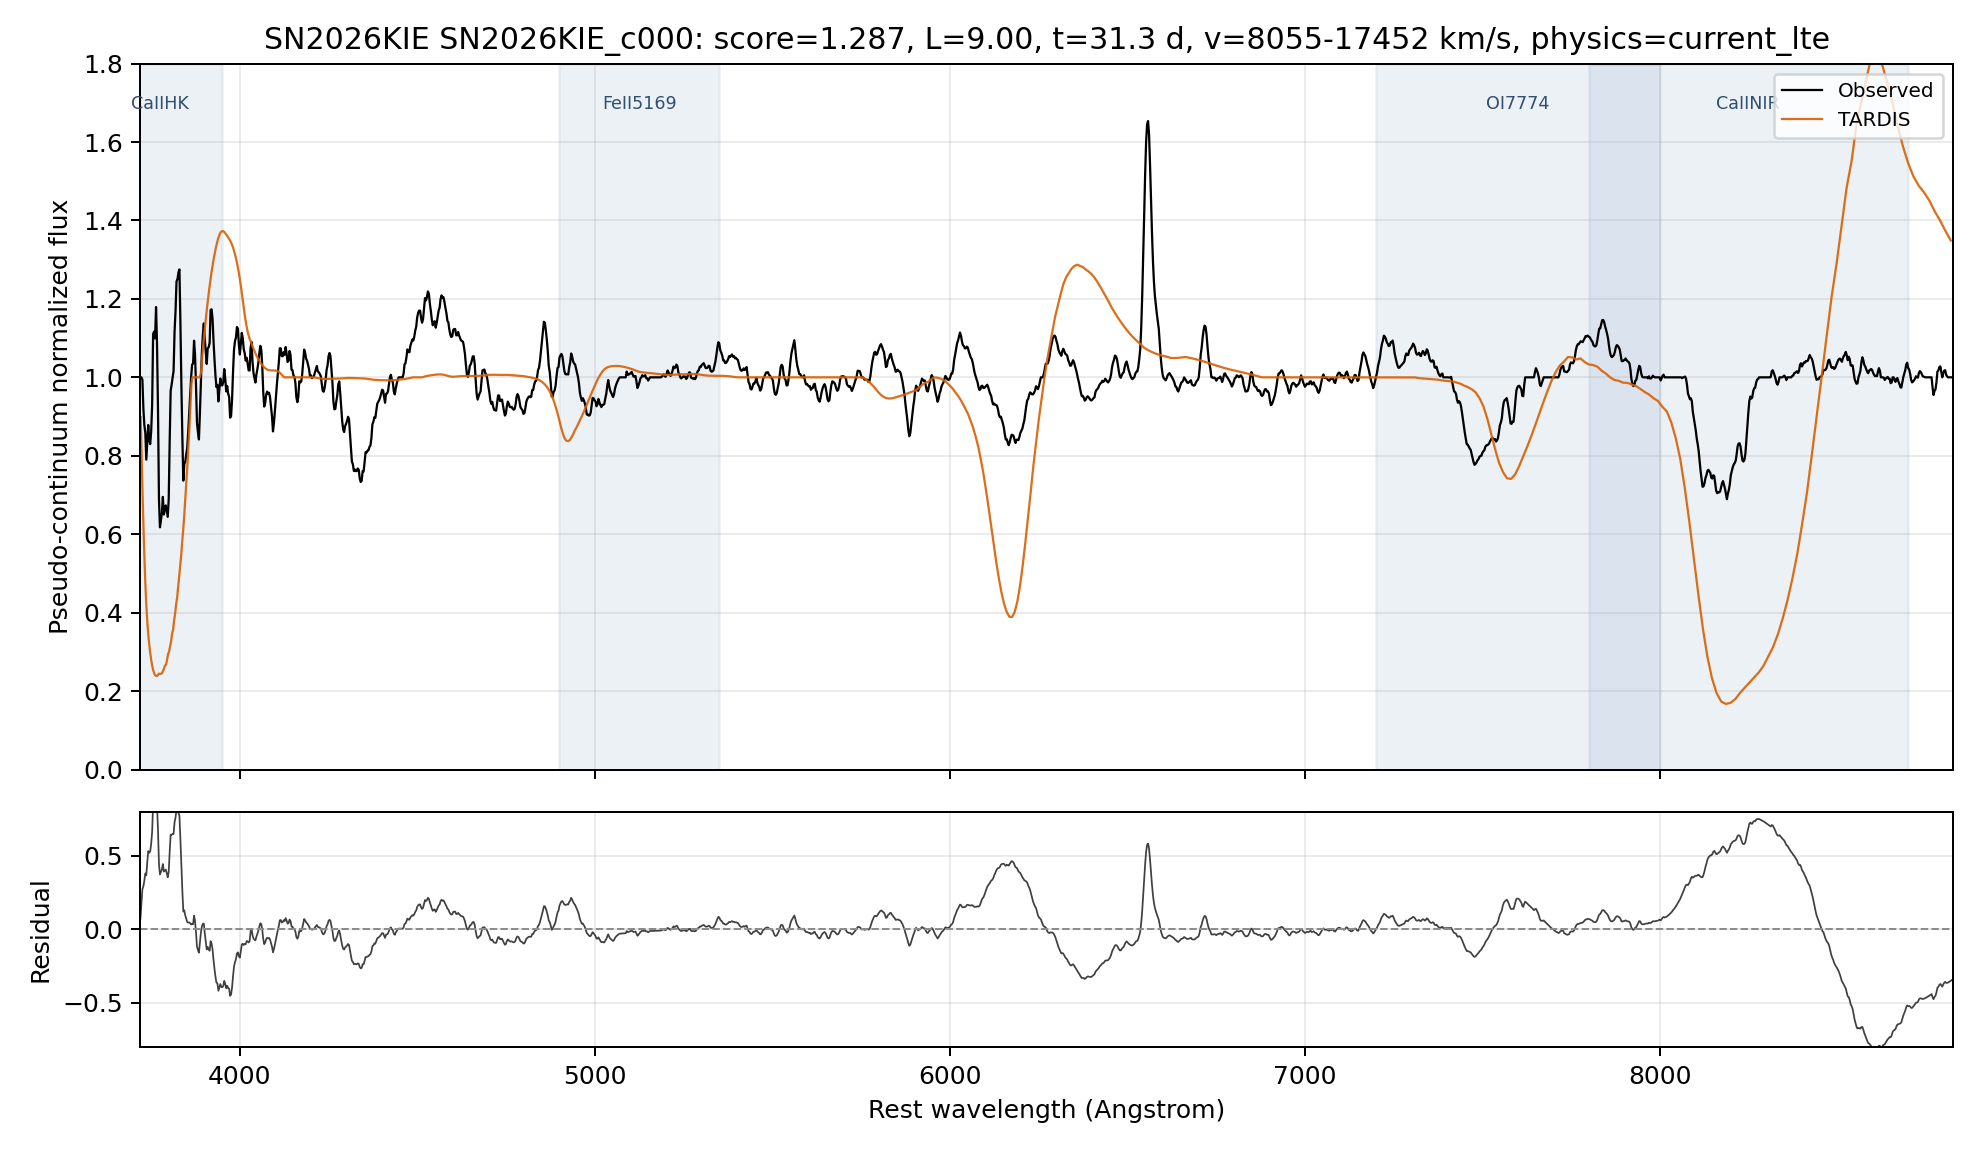
\includegraphics[width=0.95\linewidth]{images_zzzaurak/tardis_comparison_SN2026KIE.png}
\caption{SN2026KIE 的 TARDIS 定性比较。模型可部分复现 O I 与 Ca II 区域，但仍不适合做强物理参数解释。}
\label{fig:tardis-kie}
\end{figure}

总体来说，TARDIS 与前面的经验谱线测量是互补关系。经验测量给出速度、pEW、FWHM 和 QC 表，是本节主要定量结果；TARDIS 用来检查这些谱线识别和速度范围是否能由合理的一维 ejecta 模型产生。最终科学结论仍应优先引用前面的 adopted line table；TARDIS 图适合作为报告中的定性辅助图。

\subsection{本节结果的限制}
\begin{enumerate}[leftmargin=1.4em]
    \item 本节从已归约一维光谱开始，未重新做二维光谱归约；我们对其中产生的误差等细节并不清晰。
    \item 谱线速度依赖 TNS 红移。缺红移的 SN2026LMP 不做定量采用。
    \item 最低点法比高斯拟合更直接，但仍依赖窗口、平滑尺度和连续谱定义；宽线混合处的 pEW 系统误差可能明显大于表中形式误差。
    \item TARDIS 模型只拟合每颗超新星的一条代表性光谱，丰度为简化 preset，没有进行多历元联合拟合或真实分层丰度反演。
    \item 本节只给出稀疏光谱下的经验诊断和定性辐射输运检查，不等价于完整物理拟合；TARDIS 结果应作为辅助而非主证据。
\end{enumerate}

\section{结论}

\printbibliography[title={参考文献}]

\end{document}
